\chapter{Style Analyser}
\label{cap:analyser}

\chapterquote{- Marty McFly: Wait a minute, Doc. Ah... Are you telling me you built a time machine... out of a DeLorean?\\- Dr. Emmett Brown: The way I see it, if you're gonna build a time machine into a car, why not do it with some style?}{Back to the Future (1985)}

When proposing a model for stylometric analysis of e-mails for recipient-based personalised writing, it is necessary to define parameters which determine and describe the writing style of a user. For this purpose, we have developed a style analyser that extracts the messages written by the user and obtains the value of various metrics from them. Then it will be useful for analysing different user's e-mails and drawing conclusions about what parameters describe the writing style of each person more accurately.

In this section we explain the architecture of this analyser (see Section \ref{section:stylearch}) and each of the modules that compose it (they are explained in Sections \ref{section:extmod} to \ref{sect:analyserclass}). Finally, we present the behaviour of the execution with the Gmail account that is analysed (this discussion can be looked up in Section \ref{section:exebehav}).

\section{Architecture} \label{section:stylearch}
The first step when we are designing a system's architecture is to know its input and output. In this case, we want to implement a natural language processing system that analyses the writing style of e-mails. As we have previously mentioned, the stylometric analysis will be represented through chosen style markers. Therefore, our system's output is going to be that chosen metrics (they are explained in section \ref{section:measmod}) of each message.

In respect of the system's input, because of the nature of the problem we face, it is reasonable to think that it must be an e-mail. However, we do not have the corpus of e-mails to analyse. For this reason, our first step will be to extract the e-mails that will be analysed. Hence, our system's input is going to be the information of the Gmail user for accessing to the data that we are interested in. Therefore, we are going to develop a system which receives some information of a Gmail user as input and obtains different metrics for each message sent by the given user as output.

Once we clearly know the input and output of our system, we need to define the different steps that a message have to take for being analysed. In this manner, we are going to design a pipeline architecture with four different phases (extraction, preprocessing, typographic correction and measuring) as Figure \ref{fig:arch} shows. Thus, we divide the original job in four different and more simple tasks with distinct inputs and outputs required. This division into phases addresses both the need to atomise each of the steps to obtain the desired output, and to take advantage of benefits that a single indivisible system does not provide. One of these advantages is the possibility of working in parallel with each of the different phases. Another advantage, without a doubt, is the greater facility for the correction of errors in the pipeline. Thus, if an error of any kind is found in any phase, this will not affect the implementation of subsequent phases and it will not be necessary to modify the entire system. This, together with the fact that each phase stores its corresponding output using different Mongo DB documents (see Section \ref{sect:mongo}), allows us to change the behaviour of a phase (either in case of improvement or error correction of the implementation) avoiding to execute again the previous phases to the modified one, it would only be necessary to execute the changed phase and the ones that follow. Finally, it is also important to note the advantage of reusing each of the phases separately without having to rely on the others.

\begin{figure}[h]
	\centering%
	\centerline{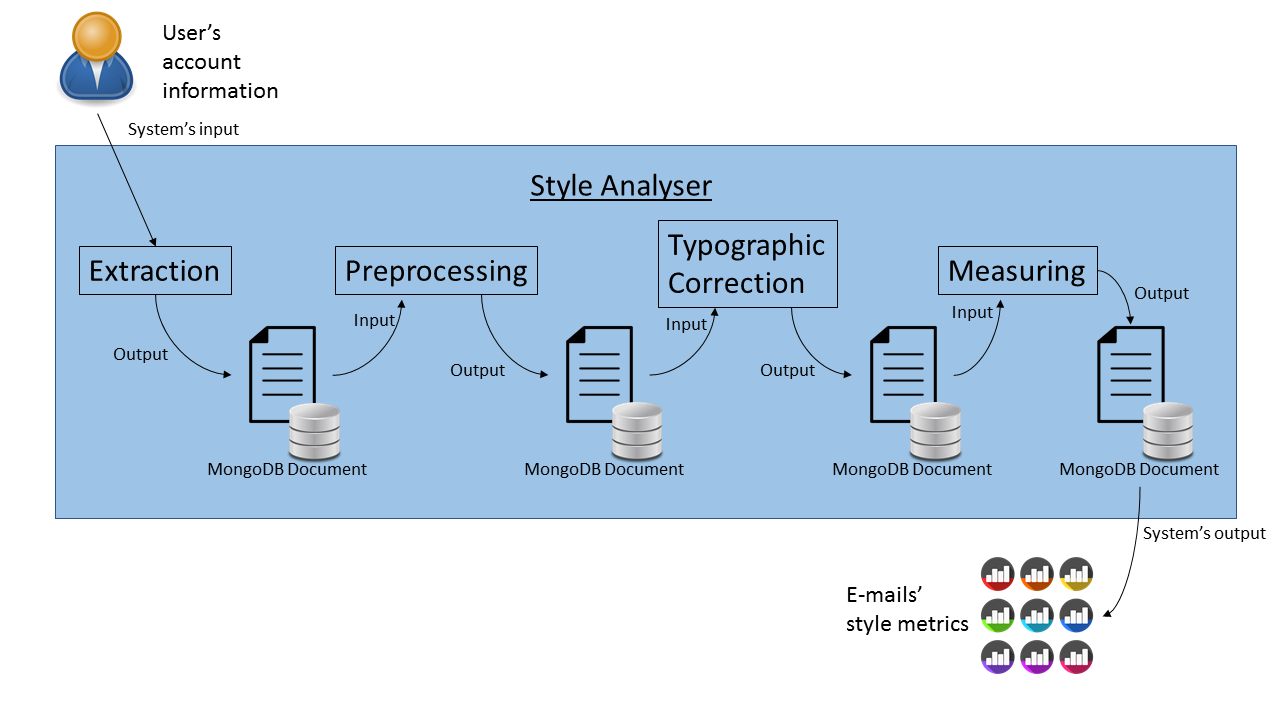
\includegraphics[width = 1.2\textwidth]{Imagenes/Bitmap/Analyser/architecture.png}}%
	\caption{Pipeline architecture of the style analyser}%
	\label{fig:arch}
\end{figure}

As it is easy to deduce, each of these phases is going to be developed as a different module. This implementation will have the advantage that each module is going to be able to work independently from the other modules, which will allow them to work in parallel. That is to say, while a message is being extracted, other e-mails could be being preprocessed, corrected or measured if they have gone through the previous phases. This optimizes the time it takes for a message to be extracted until the respective metrics are calculated (it does not have to wait for the others to move to the next phase of the pipeline). In addition, the last three (preprocessing, typographic correction and measuring) have been implemented as web services using Flask (see Section \ref{sect:flask}), which facilitates their reuse even separately in other works and projects. Let us now briefly explain what each of the defined phases consists of.

The first step, extraction phase, consists of the extraction of each one of the sent messages of the given user. In this task, we are going to take advantage of all the studied concepts about the Gmail API (see Section \ref{ssect:gmailapi}) and make use of every resource it provides us. Besides, we will try to minimize the consumed quota units in each extraction, which means we will only make the requests to the Google Servers that are strictly necessary. This first step is not just the task of extracting the resource that represents each sent message from the user's account, but also the job of transforming it to the format that the preprocessing module needs. Hence, the input of this module will be the same input as that of the complete system (information about Gmail user) and its output will be an extracted message ready for being preprocessed.

As for the second step, the preprocessing phase, consists of modifying the extracted message so that it can be interpreted by the spaCy's natural language processing model to be used. Some of the changes that a message could suffer in this phase are: the removal of the signature, the disposal of the replied messages which appears under the text, the elimination of soft break lines that quoted-printable codification (see Section \ref{sssect:quot-p}) introduce in some messages, etc. This module also addresses the need to remove characters and structures that do not correspond to those used in a plain text such as bold or italic type styles, font sizes and fonts, enumerations or bulleted lists, etc. Likewise, its output is a message with its body as a plain text.

In the implemented metrics (as we will see in section \ref{section:measmod}) we will not take into account typographical errors (such as a spelling mistake). So we will need to fix them as much as possible, and this is the typographic correction module's task. In the same way, it is possible that some tokens do not belong to our spaCy model's vocabulary. Therefore, it will be necessary to know lexical-syntactic information about the token, such as its part of speech and its lemma. These are the task of the typographic correction module.

Finally, the measuring module is in charge of calculating all the style features chosen for this work. For that purpose, it receives a message (extracted by the extracting module) with a plain text format (thanks to the preprocessing module) free from typographic error (thanks to the typographic correction module) and obtains the result of measuring all the style markers selected in the given message.

As we have explained, the input of the extracting module is information about a Gmail user and the input of the rest of the modules is a single message. However, each module is independent from each other, which means that it is necessary to have a way of assembling all this modules. For this purpose, the \textit{Analyser} class is developed (see Section \ref{sect:analyserclass}). This entity is in charge of sending to each module the required input in order to obtain its output. Moreover, it presents the system to the user, communicates the information and captures the user's information (it performs a previous filtering to check that there are no formatting errors), such as the typographic correction of the errors found. In this manner, the architecture of our style analyser system is as shown in Figure \ref{fig:umlarch} (in the following sections we will delve into each module of this system), which represents the UML (Unified Modelling Language) class diagram of it. In this figure we have avoided including both attributes and methods of each class, since with it we want to show the general structure of the system. In the sections corresponding to each of the packages and the \textit{Analyser} class, their attributes and methods will be specified and explained.

\begin{figure}[p]
	\centering%
	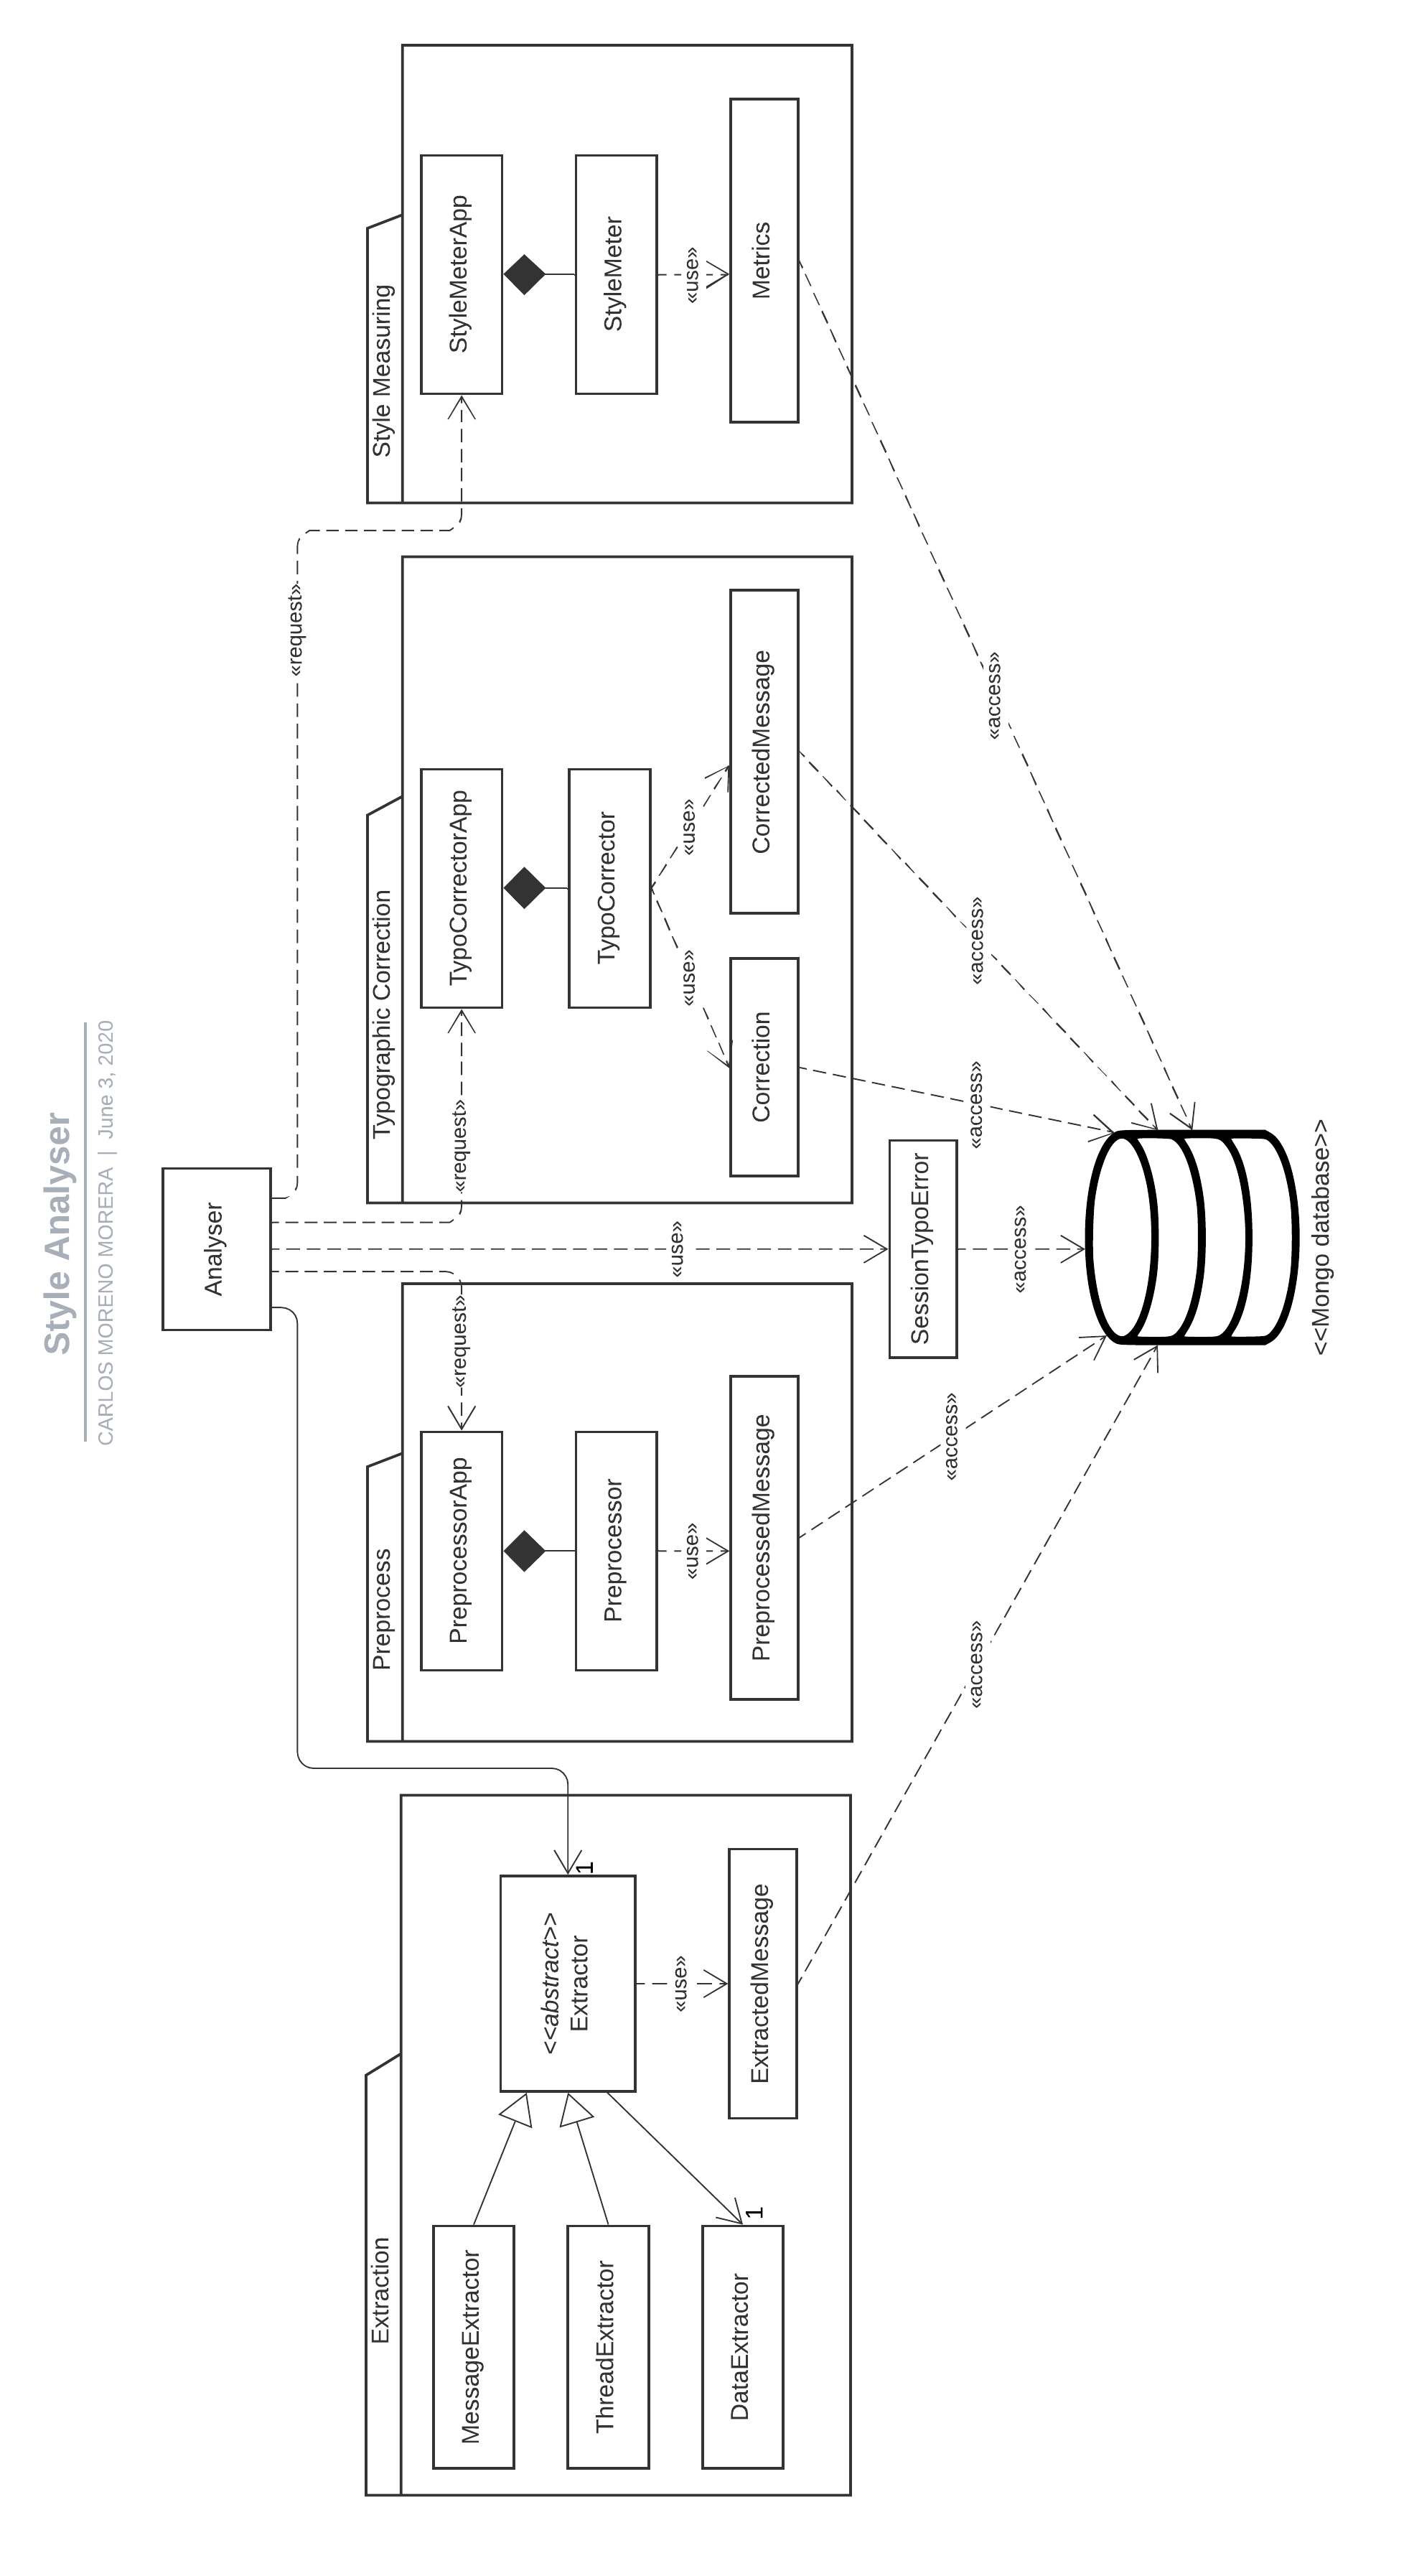
\includegraphics[height=0.85\paperheight]{Imagenes/Bitmap/Analyser/StyleAnalyserUML.png}%
	\caption{UML class diagram of the style analyser}%
	\label{fig:umlarch}
\end{figure}

As we wanted, the \textit{Analyser} manages the communication between each UML package (which represent each of the mentioned modules). Thus, this UML class will transport the output of each module to the input of the subsequent phase so as to fulfil the pipeline established in Figure \ref{fig:arch}.

If we look at the relationship shared by the \textit{Analyser} class and the \textit{Extraction} package (specifically with the \textit{Extractor} class of this module), we will notice that it is an uni-directional binary association, what it means that the objects of the second are connected with the objects of the first. Furthermore, we can observe a multiplicity index in the arrowhead (the \textit{Extraction}'s end), which means that the \textit{Analyser} will be related with an only \textit{Extractor} object (it will not be necessary to have more than one \textit{Extraction} package in order to obtain all user's sent messages).

The rest of packages are ``used'' by the \textit{Analyser}, through a POST HTTP request, because all of them are implemented as web services. It contacts with the module's app which is related with the module's main class (which is in charge of carrying out its corresponding task).

An important observation to mention is the fact that all packages interact with their corresponding classes, which act as DAO (Data Access Object), with the database used (with Mongo DB technology as it is explained in Section \ref{sect:mongo}). Their interaction is based on storing their results in it. The main advantage of this implementation is that it is not required to have enough dynamic memory in order to process every message at the same time. In addition to it, as we have explained, if an error is detected in an specific phase, it is not necessary to execute the previous modules again. With this in mind, it is reasonable to think that each module's main class, of the last three phases, will make use of the corresponding class with the purpose of saving its result, obviously after finishing its execution with the given message.

Below we only have to enter in detail of each of the packages and of the \textit{Analyser}, in order to completely understand the style analyser.

\section{Extraction module} \label{section:extmod}
The extraction module encapsulates all the necessary functionality in order to extract the given user's sent messages. As it is shown in Figure \ref{fig:umlext}, this UML package has five different UML classes: \textit{Extractor}, \textit{MessageExtractor}, \textit{ThreadExtractor}, \textit{DataExtractor} and \textit{ExtractedMessage}.

\begin{figure}[p]
	\centering%
	\centerline{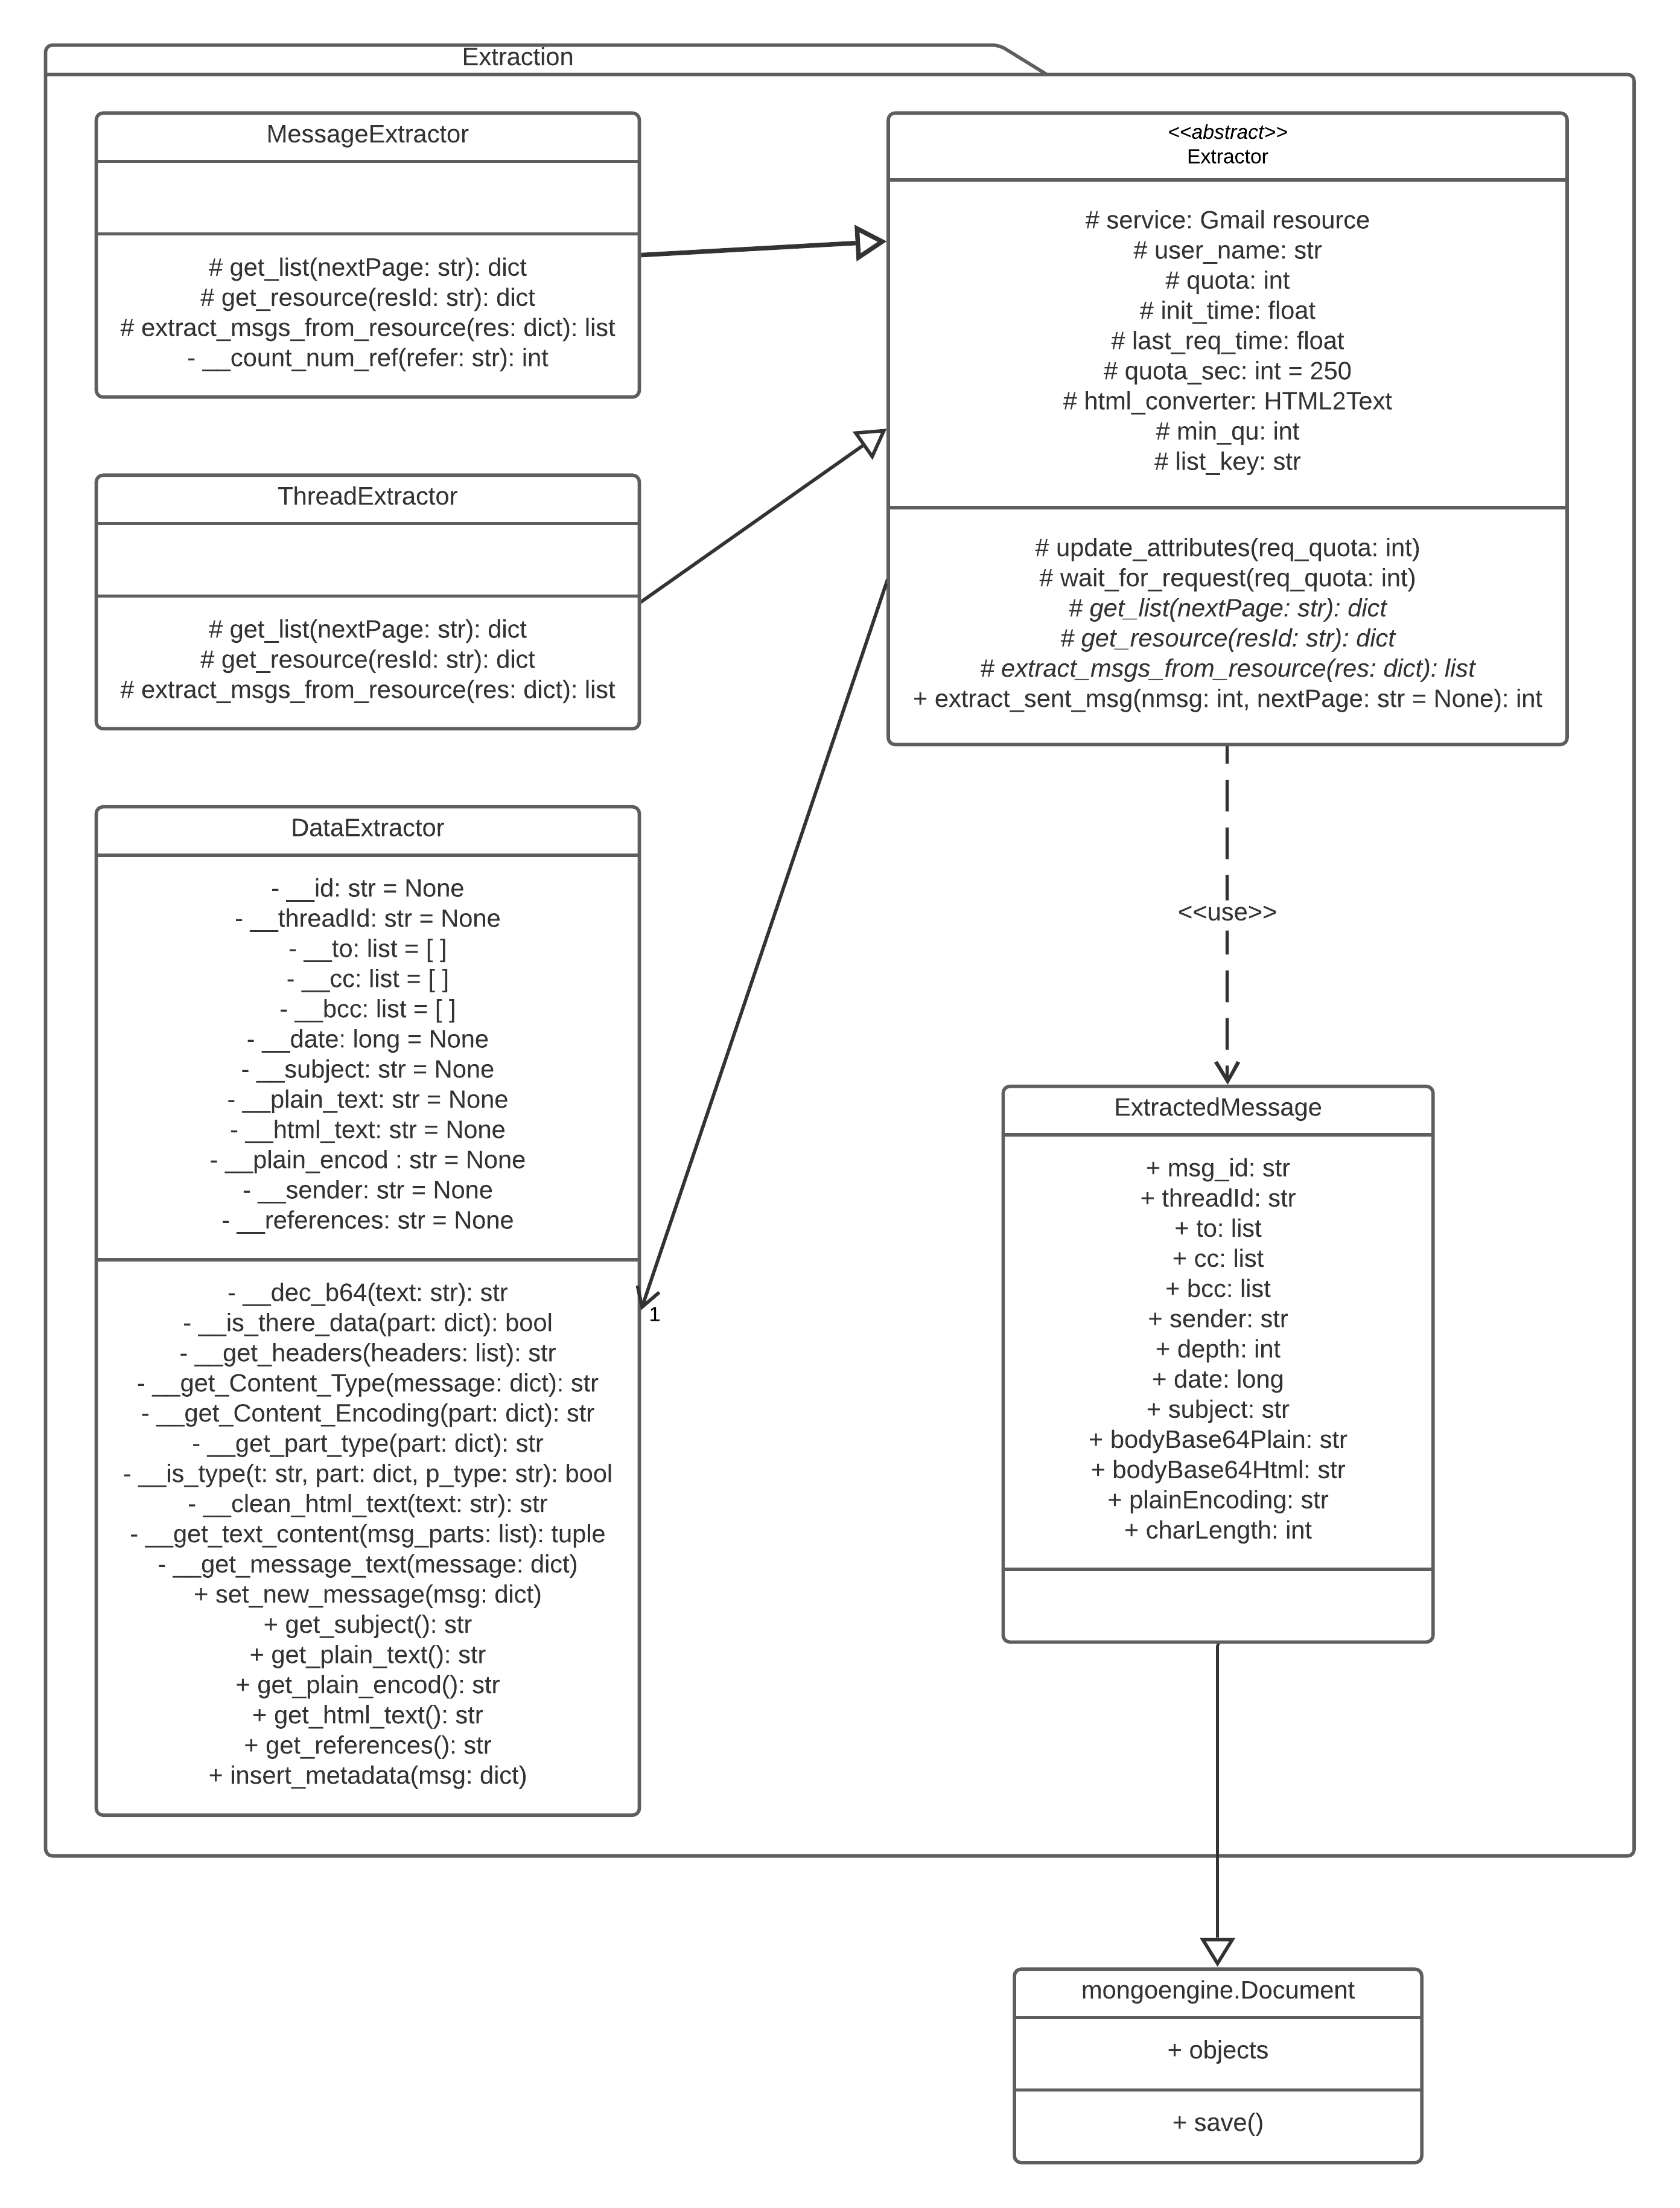
\includegraphics[width=0.9\paperwidth]{Imagenes/Bitmap/Analyser/extractionUML.png}}%
	\caption{UML class diagram of the extraction module}%
	\label{fig:umlext}
\end{figure}


The main class of the above five is the \textit{Extractor} class, which is an abstract class implemented by \textit{MessageExtractor} and \textit{ThreadExtractor} classes. The reason for implementing it as an abstract class with the abstract methods \textit{get\_list}, \textit{get\_resource} and \textit{extract\_sent\_msg}, lies in the desire to minimise the number of quota units used during this process. Let's explain this in detail.

As we have see in the Table \ref{tab:quotaUnits}, to carry out the messages resource's operation costs five quota units and to perform the same operations for the thread's resource costs ten quota units. However, when the operation \textit{messages.get} is invoked we get a single message, whereas when the operation \textit{threads.get} is called we get as many messages as there are in the thread. Therefore, minimising the amount of quota units used depends on the number of messages and threads we have.

When we are in the extraction process, at first it is necessary to invoke a \textit{list} method. It will return a list of, at least, 100 identifiers of the resource (message or thread). Then, these identifiers will be used to obtain (by calling the corresponding \textit{get} method) each of the listed resources. If we want to obtain the identifiers of the remaining resources, we will have to invoke \textit{list} again with the \textit{nextTokenPage} obtained in the previous call. With this in mind, we are going to invoke the corresponding \textit{list} method as many times as the result of applying the ceiling function to the division of the number of resources by 100; and we are going to invoke the corresponding \textit{get} method as many times as the amount of resources the user has (this number is possible to know by calling the \textit{get} method of the labels resource and giving it the string value \textit{SENT} as its parameter called \textit{id}, which only consumes one quota units each time). Hence, the number of quota units inverted in an extraction process will be determined by the following formula:

$$
Q = L\cdot\left\lceil\frac{N}{100}\right\rceil+G\cdot N
$$

Where $L$ is the cost in quota units of invoking the corresponding \textit{list} method once, $N$ is the number of resources that the user has and $G$ is the cost in quota units of calling the corresponding \textit{get} method once. It is important to remember that the division is the integer and not the real one.

Following the previous expression and the quota units cost of Table \ref{tab:quotaUnits}, we are able to claim that the number of quota units inverted in a message extraction process will be:

$$
Q_M = 5\cdot\left\lceil\frac{N_M}{100}\right\rceil+5\cdot N_M
$$

Where $N_M$ is the amount of sent messages that the user has. However, the cost in quota units of a thread extraction process will be determined by:

$$
Q_T = 10\cdot\left\lceil\frac{N_T}{100}\right\rceil+10\cdot N_T
$$

Where $N_T$ is the number of sent threads that the user has. Consequently, when we obtain that $Q_M < Q_T$, we will save more quota units by executing a message extraction process and, when $Q_T < Q_M$, it will happen by executing a thread extraction process.

Returning to the extraction module, even though the choice between the two types of extraction is done by the Analyser (see Section \ref{sect:analyserclass}), it is necessary to implement both possibilities. For this reason, \textit{Extractor} class was implemented as an abstract class with the methods related to the \textit{list} and \textit{get} functions of the Gmail API: \textit{get\_list} (which calls the corresponding \textit{list} method) and \textit{get\_resource} (which invokes the corresponding \textit{get} method). In addition to them, we can find the \textit{extract\_msgs\_from\_resource} as an abstract method. This function is in charge of extracting the necessary information from the corresponding resource in order to obtain a list of messages (in the case of the message resource the list has only one item) which are going to be stored in the database. In other words, it transforms a message (or a thread of messages) with the structure explained in Section \ref{sssect:msgres} into the following structure (in the case of the thread resource each message will be transformed to the following structure):

\begin{python}
{
	'id' : string,
	'threadId' : string,
	'to' : [ string ],
	'cc' : [ string ],
	'bcc' : [ string ],
	'sender' : string,
	'depth' : int,               # How many messages precede it
	'date' : long,               # Epoch ms
	'subject' : string,
	# Body as plain text encoded using base64
	'bodyBase64Plain' : string,
	# Body as html text encoded using base64
	'bodyBase64Html' : string,
	# Original encoding of the body as a plain text
	'plainEncoding' : string,    
	'charLength' : int
}
\end{python}

Once the message has this structure, it is ready to be saved in the database, because of, as we can observe in Figure \ref{fig:umlext}, the dictionary keys are the same as the attributes of the \textit{ExtractedMessage} class (which inherits from the \textit{mongoengine.Document} class, allowing it to insert elements in the database). Indeed, the \textit{extract\_msgs\_from\_resource} method returns a list of \textit{ExtractedMessage} objects.

In addition to the explained abstract methods, in the \textit{Extractor} class we can find the \textit{extract\_sent\_msg}, which is in charge of the extraction algorithm that we mentioned before (invoke the corresponding \textit{list} method, for each identifier get the resource, call the function \textit{extract\_msgs\_from\_resource}, etc.). During this process, the \textit{Extractor} must check that it does not exceed the set limit of quota units, both the daily limit and the secondly limit. Once the daily limit is reached, the process must stop. In the case of the secondly limit, the \textit{Extractor} must stop and wait until it can continue using the Gmail API operations. This is the task of \textit{update\_attributes} (which updates the time and quota attributes such as \textit{quota}, \textit{quota\_sec}, \textit{last\_req\_time} and \textit{init\_time}) and \textit{wait\_for\_request} methods.

In respect of the \textit{Extractor} class, there is an only remaining detail that should be mentioned. It has an attribute called \textit{html\_converter}. This attribute is an object of the \textit{HTML2Text} class from \textit{html2text} Python's library\footnote{\url{https://pypi.org/project/html2text/}}, which is used in order to obtain the message body as a plain text from the e-mail body as HTML text in the event that there is a lack of first one.

If we observe the \textit{Extraction} package, we will also find the \textit{DataExtractor} class, which is related with the \textit{Extractor} class by an uni-directional binary association with a multiplicity index in the arrowhead (the \textit{DataExtractor}'s end). It performs the task of extracting the information of a given e-mail. To this end, it goes through the headers list (where information as the recipient can be found) and the MIME message parts tree studied in Section \ref{sssect:MIMEheaders}, in order to get the message body. Likewise, once an e-mail is extracted from Gmail API, the \textit{DataExtractor} class receives it and acquires all the required information from it.

\section{Preprocessing module} \label{section:prepmod}
The preprocessing module receives the message with the structure given by the extraction module and modifies the e-mail so that it can be interpreted by the spaCy's pretrained model. As it is shown in Figure \ref{fig:umlprep}, this UML package has three different UML classes: \textit{PreprocessorApp}, \textit{Preprocessor} and \textit{PreprocessedMessage}.

\begin{figure}[p]
	\centering%
	\centerline{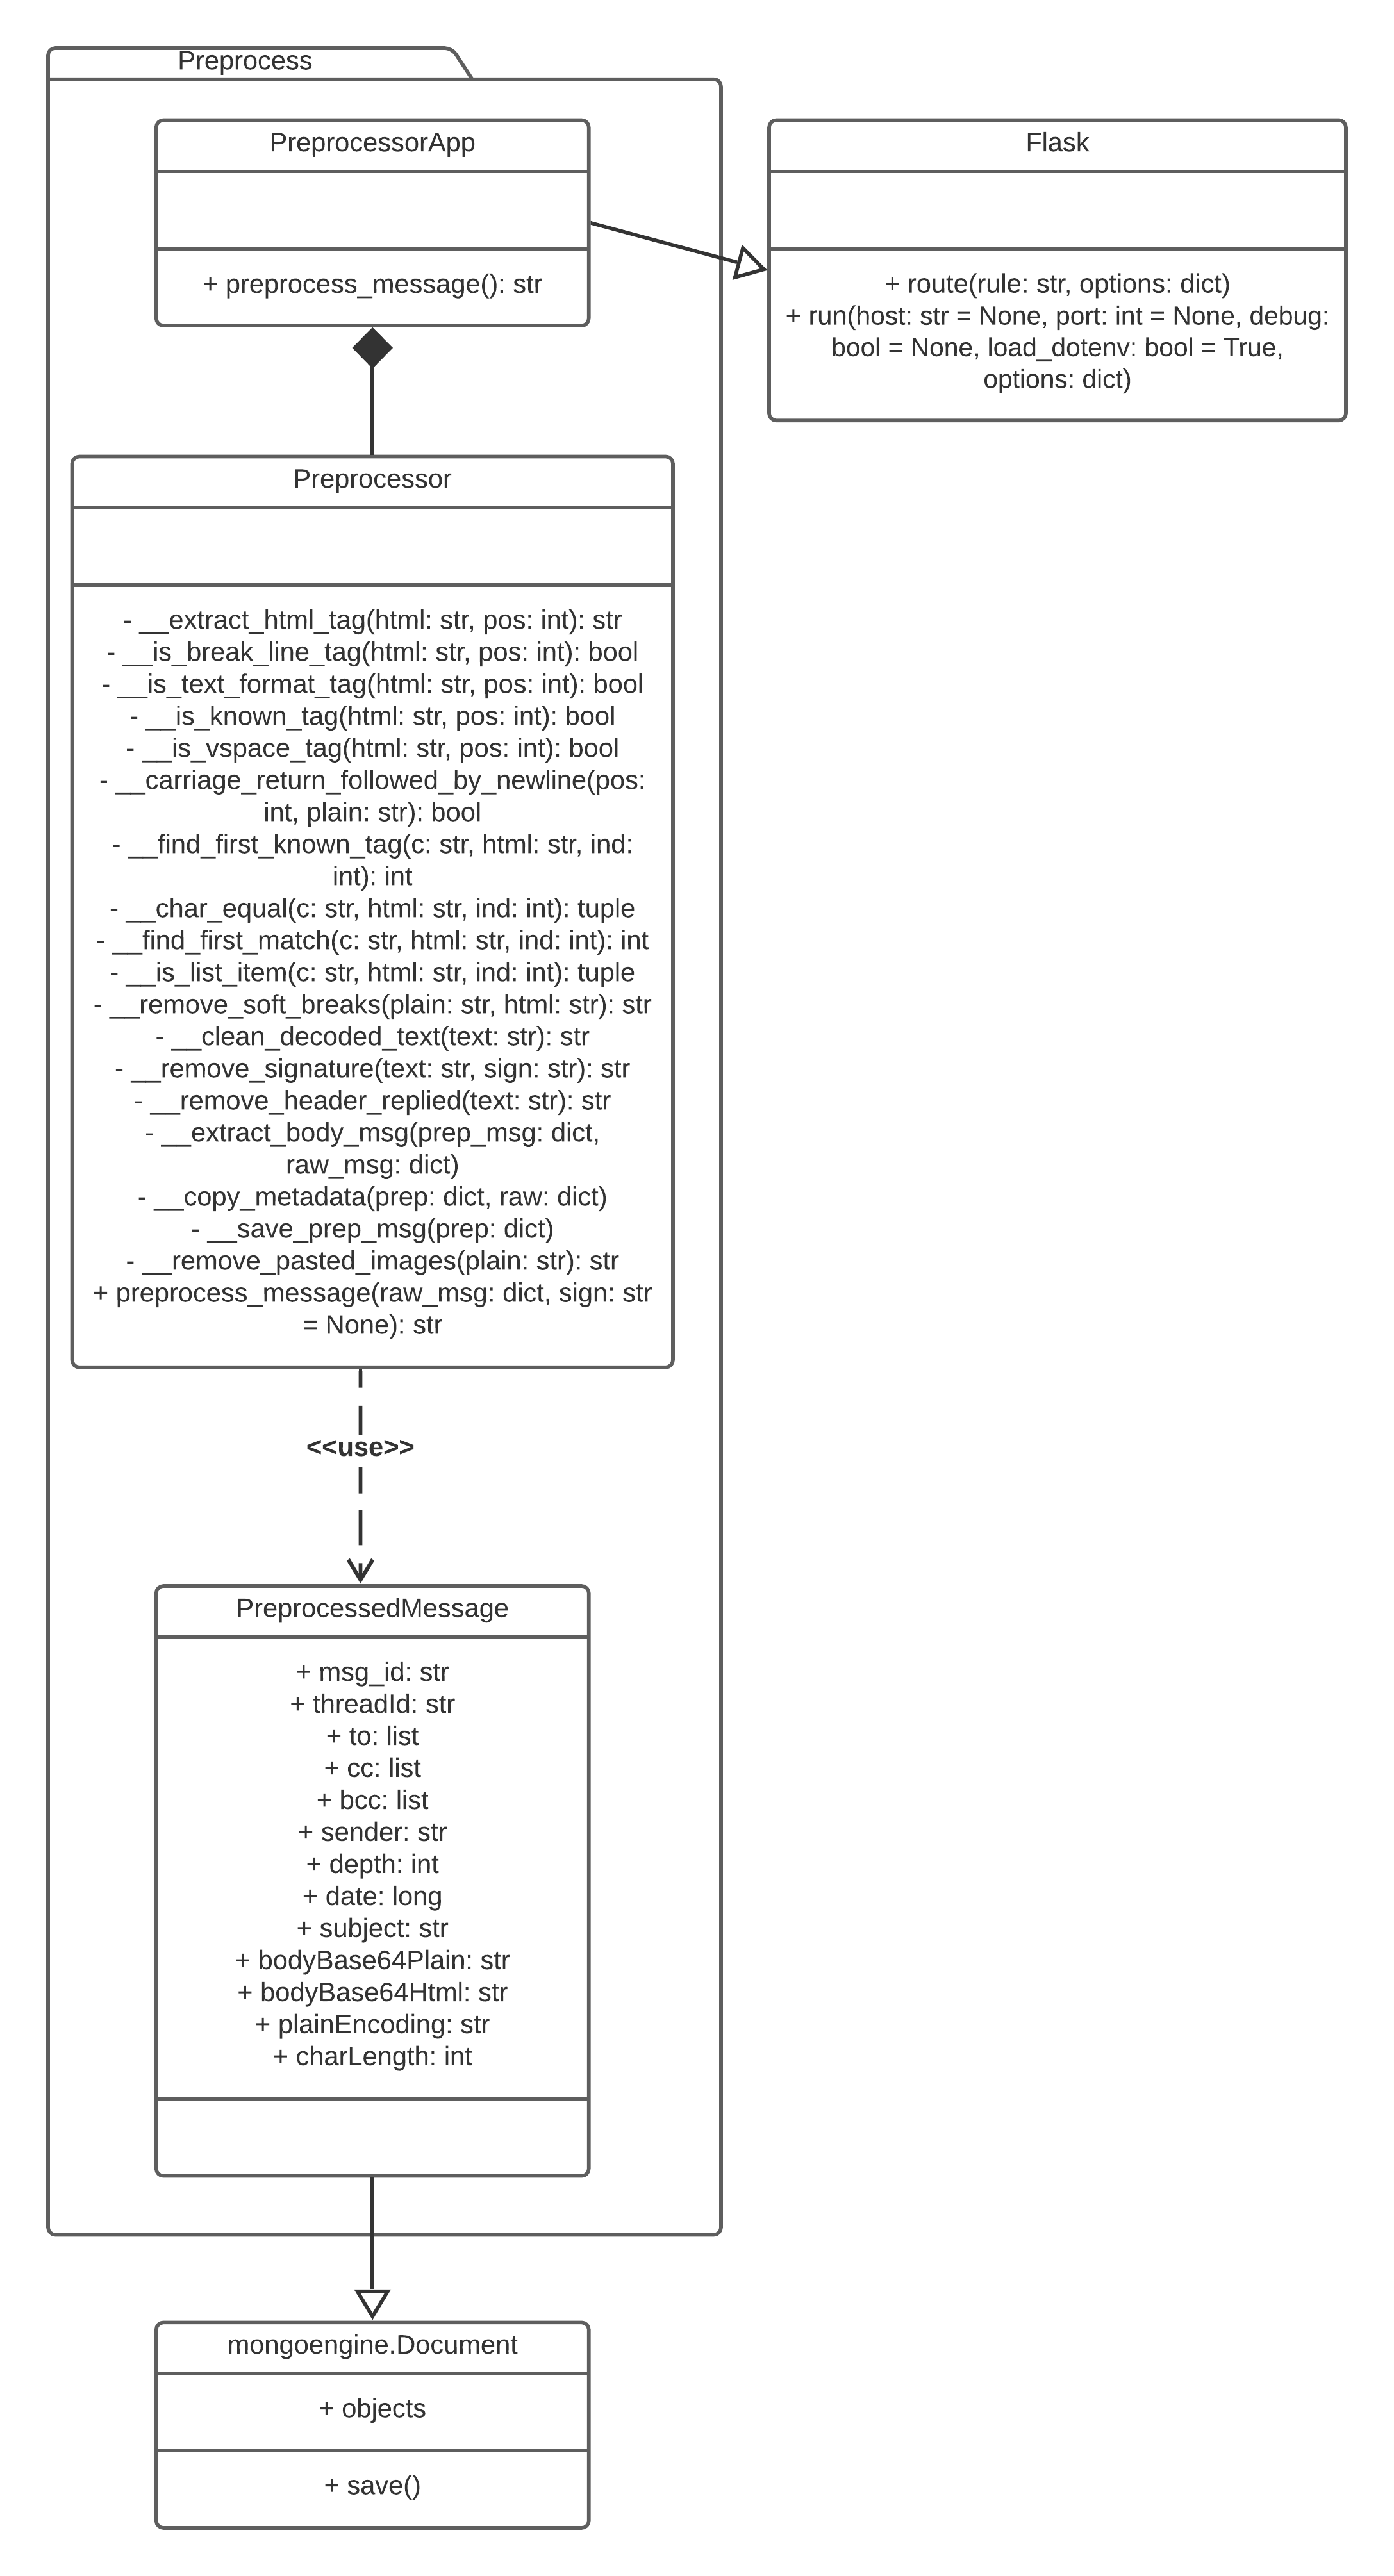
\includegraphics[height=0.85\paperheight]{Imagenes/Bitmap/Analyser/preprocessUML.png}}%
	\caption{UML class diagram of the preprocessing module}%
	\label{fig:umlprep}
\end{figure}

First of all, we can observe the \textit{PreprocessorApp} class. It inherits from \textit{Flask} class (see Section \ref{sect:flask}), which implements a simple web service. Consequently, if we want to preprocess a message, it will be necessary to execute a POST HTTP request with the e-mail as a \textit{json} in it. Having done so, the \textit{preprocess\_message} method will be invoked and send the given message structure to the \textit{Preprocessor} class by calling its only public method: \textit{preprocess\_message}. There is also the possibility of transmitting the user's e-mail signature to the \textit{Preprocessor} (so that it can be removed from the different messages) by including it as an string in the sent \textit{json}.

The main class of this UML package is the \textit{Preprocessor} class. It is in charge of modifying the given message. For this reason, it has different methods which implements the distinct tasks that it has to carry out.

The first task this module performs is to filter those e-mails whose message body as plain text is empty, which means that they lack the \textit{bodyBase64Plain} field. As our purpose is analyse the writing style of the user, we are not interested in e-mails without text. Thus, these messages are discarded.

Then, the images inserted in the message body (not as an attachment) are removed by calling the \textit{\_\_removed\_pasted\_images} method. This function make use of the simple Python's regular expression \pythoninline{r'\\[image:[\^\\]]+\\]'}, detects the position of the different images with it and takes them away.

Once pasted images are removed, the \textit{\_\_extract\_body\_msg} method removes the text of replied e-mail (if it exists) and the soft break lines inserted in the body, as a consequence of the established format in \cite{rfc2646}. When someone replies an e-mail from a Gmail account, the replied message is automatically included under the response (indeed it is possible to intersperse the answer and the responded text). As it is not a written composed by our user, this copied text must be taken away. To this end, the \textit{Preprocessor} class creates an object of the \textit{EmailReplyParser} class of the \textit{email\_reply\_parser}\footnote{\url{https://pypi.org/project/email_reply_parser/0.1.0/}} Python's library. With its \textit{parse\_reply} method, only the response is obtained with the replied message's header automatically included (\textit{EmailReplyParser} class does not remove it). However, such header is easy to detect by using regular expressions, due to it has an specific format as the following line (written in Spanish):

\textit{El mié., 27 may. 2020 a las 11:11, Name (<example@mailserver.com>) escribió:}

The designed regular expression detects this type of sentences with the moment (date and time) and the sender. Once \textit{Preprocessor} knows its position, it is possible to take it away.

A similar problem appears with forwarded messages. Nevertheless, unlike replied e-mails, it is not possible to detect if the user has interspersed new text in the forwarded written. For this reason, \textit{Preprocessor} detects the forwarded header, which indicates the beginning of the resent message, and deletes all the text from it.

In addition to the replied or forwarded text, we find the problem of the inserted soft break lines in order to follow the standard format for sending e-mails. We have implemented two solutions for this issue in \textit{\_\_clean\_decoded\_text} and \textit{\_\_remove\_soft\_breaks} methods. The first function deletes all soft break lines in messages encoded with quoted-printable (see Section \ref{sssect:quot-p}). The second, compares the message body as HTML text and as plain text and removes all soft break lines that do not appear as an HTML tag. Moreover, during this process we detects characters that should not appear in the plain text. For instance, Gmail delimits the text in bold with the symbol ``*'' (there are more examples as the beginning of a bulleted list, an enumeration or the change of font or font size). As in the HTML text it will appear between two tags, we recognise this fact and take the delimiter character away. In this way we are able to obtain a real plain text.

The last modification made by the preprocessor is the removal of the signature. This only happens if the user has provided it to the system, since the recognition of the signature is a complex problem that is not the objective of this work. The \textit{\_\_remove\_signature} method is is responsible for carrying out that task.

Once an extracted e-mail is preprocessed, it is ready to be saved in the database. As it happened with the \textit{ExtractedMessage} class, the \textit{PreprocessedMessage} class inherits from the \textit{mongoengine.Document} class, allowing it to insert elements in the database. If we compare the \textit{ExtractedMessage} and \textit{PreprocessedMessage} class, we will realise that they have the same attributes, so a preprocessed message has the same structure as an extracted one.

\section{Typographic correction module} \label{section:typomod}
Typographic correction module receives the message with the structure given by the preprocessing module and detects the typographic errors present in the given e-mail. As it is shown in Figure \ref{fig:umltypo}, this UML package has four different UML classes: \textit{TypoCorrectorApp}, \textit{TypoCorrector}, \textit{CorrectedMessage} and \textit{Correction}.

\begin{figure}[p]
	\centering%
	\centerline{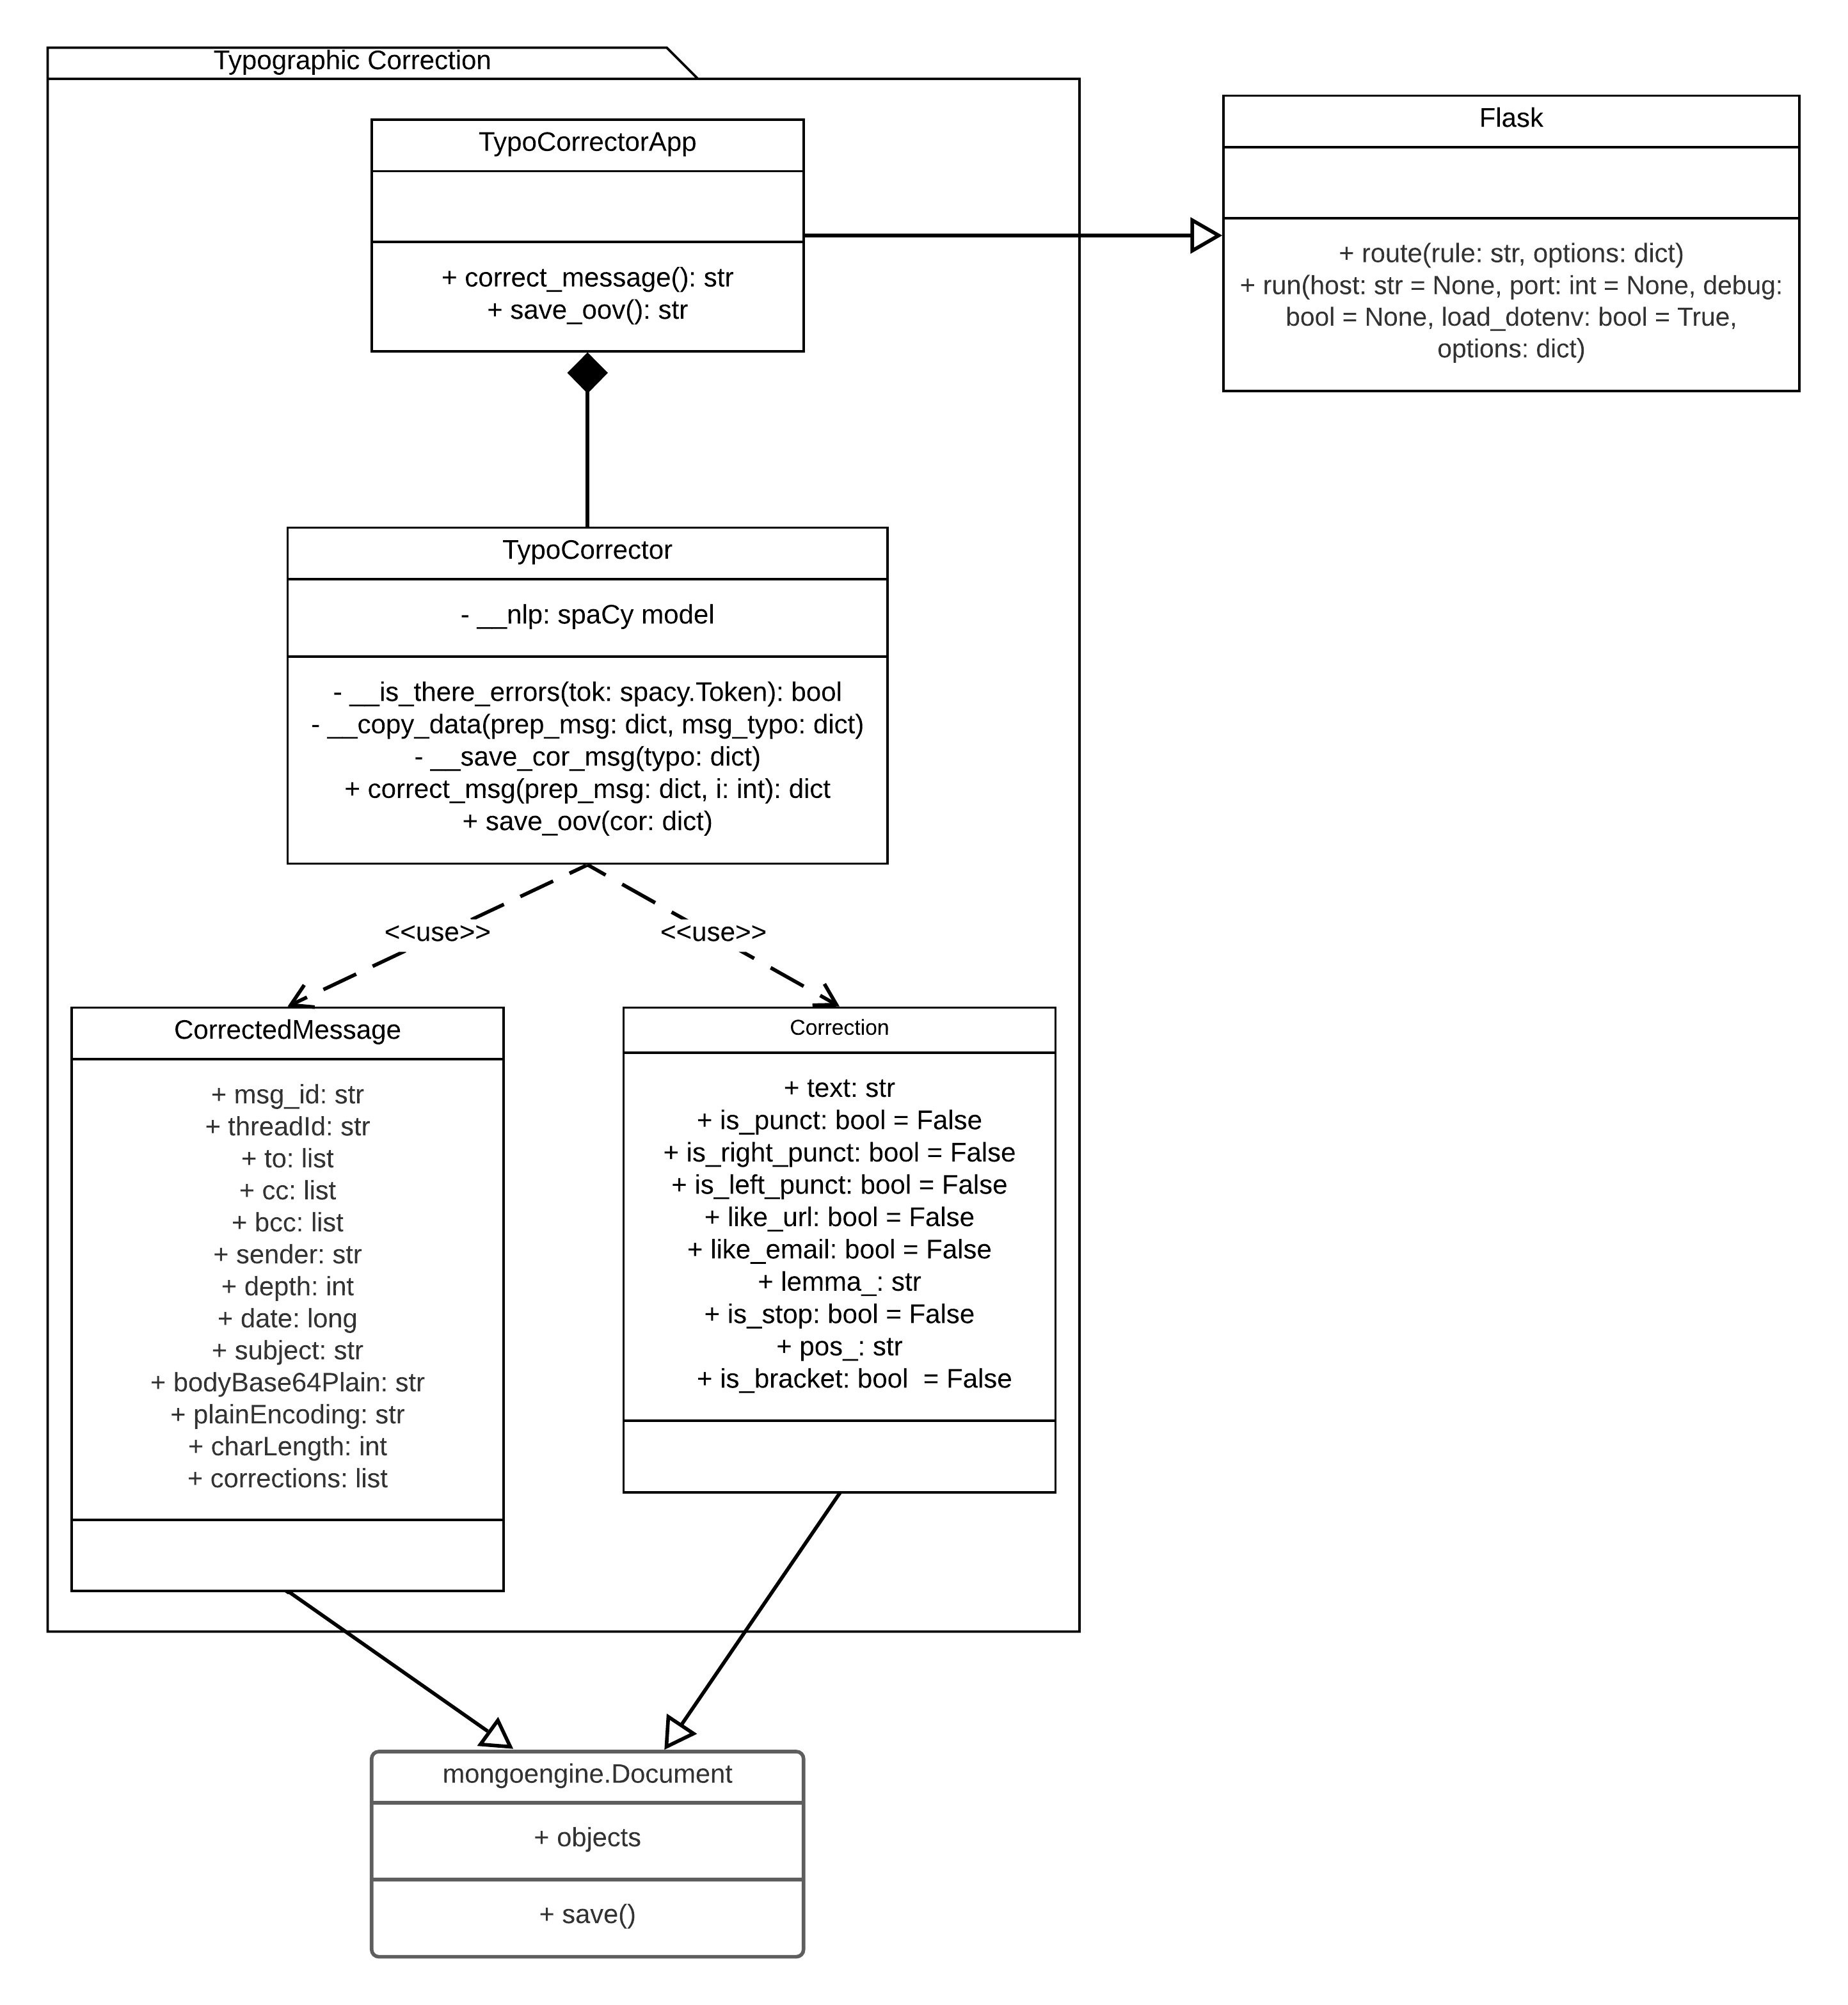
\includegraphics[width=0.9\paperwidth]{Imagenes/Bitmap/typoUML.png}}%
	\caption{UML class diagram of the typographic correction module}%
	\label{fig:umltypo}
\end{figure}

As it happened with \textit{PreprocessorApp}, \textit{TypoCorrector} inherits from \textit{Flask} class and, thanks to it, this class implements a simple web service. However, unlike \textit{PreprocessorApp}, \textit{TypoCorrector} has two different methods which carry out distinct task. These two functions correspond to the two \textit{TypoCorrector}'s public method with the same name. Thus, if we want to invoke one of these public methods, it will be necessary to execute a POST HTTP request with an e-mail, in order to be corrected (in the case of the method \textit{correct\_msg}), or with the unrecognised token (which has been wrongly classified as ``out of vocabulary'' by our spaCy's model) that is going to be saved (we will explained both tasks in detail later). Each one of them is going to have a different url address.

The main class of this UML package, as it happens with the rest of packages, is the \textit{TypoCorrector} class. It is in charge of detecting the typographic errors and correcting them if it is possible. For this purpose it makes use (as an attribute) of an spaCy's pretrained model, specifically the one called \textit{es\_core\_news\_md}\footnote{\url{https://spacy.io/models/es}}.

The first public method that we are going to explain is \textit{correct\_msg}, which receives as parameters a message and an index. The method's parameters are originally a preprocessed message with its structure and the index as 0, which indicates that the e-mail must be corrected from the beginning, because it points the word from which the typographic correction should be made. When the function finishes its operations, it returns a dictionary with the following structure:

\begin{python}
{
	'typoCode': <enum 'TypoCode'>,
	'index': int,
	'typoError': str,
	'token_idx': int,
	'message': {
		'id' : string,
		'threadId' : string,
		'to' : [ string ],
		'cc' : [ string ],
		'bcc' : [ string ],
		'sender' : string,
		'depth' : int,               # How many messages precede it
		'date' : long,               # Epoch ms
		'subject' : string,
		'bodyPlain' : string,
		'bodyBase64Plain' : string,
		'plainEncoding' : string,
		'charLength' : int,
		'corrections' : [
		{
			'text': str,
			'is_punct': bool,
			'is_right_punct': bool,
			'is_left_punct': bool,
			'like_url': bool,
			'like_email': bool,
			'lemma_': str,
			'is_stop': bool,
			'pos_': str,
			'is_bracket': bool,
			'position': int
		}
		]
	}
}
\end{python}

If no typographic errors are detected in the text or the user's help is not needed, the \textit{message} field is previously saved in the database, by using the \textit{CorrectedMessage} class (its attributes perfectly match with the fields of the \textit{message} field dictionary), the \textit{typoCode} field will take the value \textit{successful} and the \textit{typoError} and \textit{token\_idx} fields will take the value \textit{None}. However, in other case, the execution of the system changes.

The first task the \textit{correct\_msg} method performs is to filter those e-mails whose message body as plain text is empty, due to the preprocess could produce this result, such as in forwarded messages without new text. In this case, the \textit{typoCode} will take the value \textit{notAnalysed}.

Then, it checks from the given index onwards if one token is recognised by our spaCy's model as ``out of vocabulary''. If this happens, the word is searched in the database of corrections (which is easy to manage thanks to the \textit{Correction} class) in case it was previously stored in it as a non-out-of-vocabulary token (in this database we have all words that are not really a typographic error, but they are not recognised by our natural language processing model). If the word appears in it, the information of this ``correction'' is appended to the \textit{``corrections''} list (each of its elements has the same field as the \textit{Correction} class' attributes) and the execution continues as usual, as if no error has been detected.

In the other hand, if the detected out of vocabulary token is not in our \textit{Correction} database, which means that it could be a real typographic error or a existent word which is not recognised by our spaCy's model and not previously stored, the \textit{Analyser} class (out of this module), with the help of the user, will be in charge of determining if it is a real typographic error and correcting it in that case. For this reason, the \textit{TypoCorrect} will return the mentioned structured with the \textit{typoCode} field taking the value \textit{typoFound}, the \textit{word} one with the text of the detected token and the \textit{token\_idx} with the character position of the beginning of the found word. The \textit{index} field will always take the value of the position of the last analysed word, if there are no errors detected it will be the number of words in the message.

Once the \textit{Analyser} has determined if the given word is a real typographic error, and corrected it in that case, it will invoke again the \textit{correct\_msg} method, through a POST HTTP request, and it will send as a parameter the returned \textit{message} field (probably with the message body changed or with a new element in \textit{corrections} list) and with the corresponding index, for example if the detected token was not a real typographic error, the index will be the position after the word (due to the previous words has been analysed yet). This is the advantage of this function, it allows us to start a new typographic correction or continue a previously started one, because it admits as the \textit{prep\_msg} parameter a preprocessed message or a partially corrected message.

In this Section, we have explained when the \textit{Correction} queries are carried out, but we have not said anything about when its elements are inserted. For this purpose, the \textit{save\_oov} method was implemented. If the \textit{Analyser} determines that the returned word is not a typographic error, it can carry out a POST HTTP request in order to save the information of this word in the database for future cases.

\section{Measuring module} \label{section:measmod}
The measuring module is in charge of calculating all the selected writing style metrics. In order to measure these features, it receives from the \textit{Analyser} class a corrected message with the following structure (which matches with the stored messages' structure):

\begin{python}
	{
		'id' : string,
		'threadId' : string,
		'to' : [ string ],
		'cc' : [ string ],
		'bcc' : [ string ],
		'sender' : string,
		'depth' : int,               # How many messages precede it
		'date' : long,               # Epoch ms
		'subject' : string,
		'bodyBase64Plain' : string,
		'plainEncoding' : string,
		'charLength' : int,
		'corrections' : [
		{
			'text': str,
			'is_punct': bool,
			'is_right_punct': bool,
			'is_left_punct': bool,
			'like_url': bool,
			'like_email': bool,
			'lemma_': str,
			'is_stop': bool,
			'pos_': str,
			'is_bracket': bool,
			'position': int
		}
		]
	}
\end{python}

\begin{figure}[p]
	\centering%
	\centerline{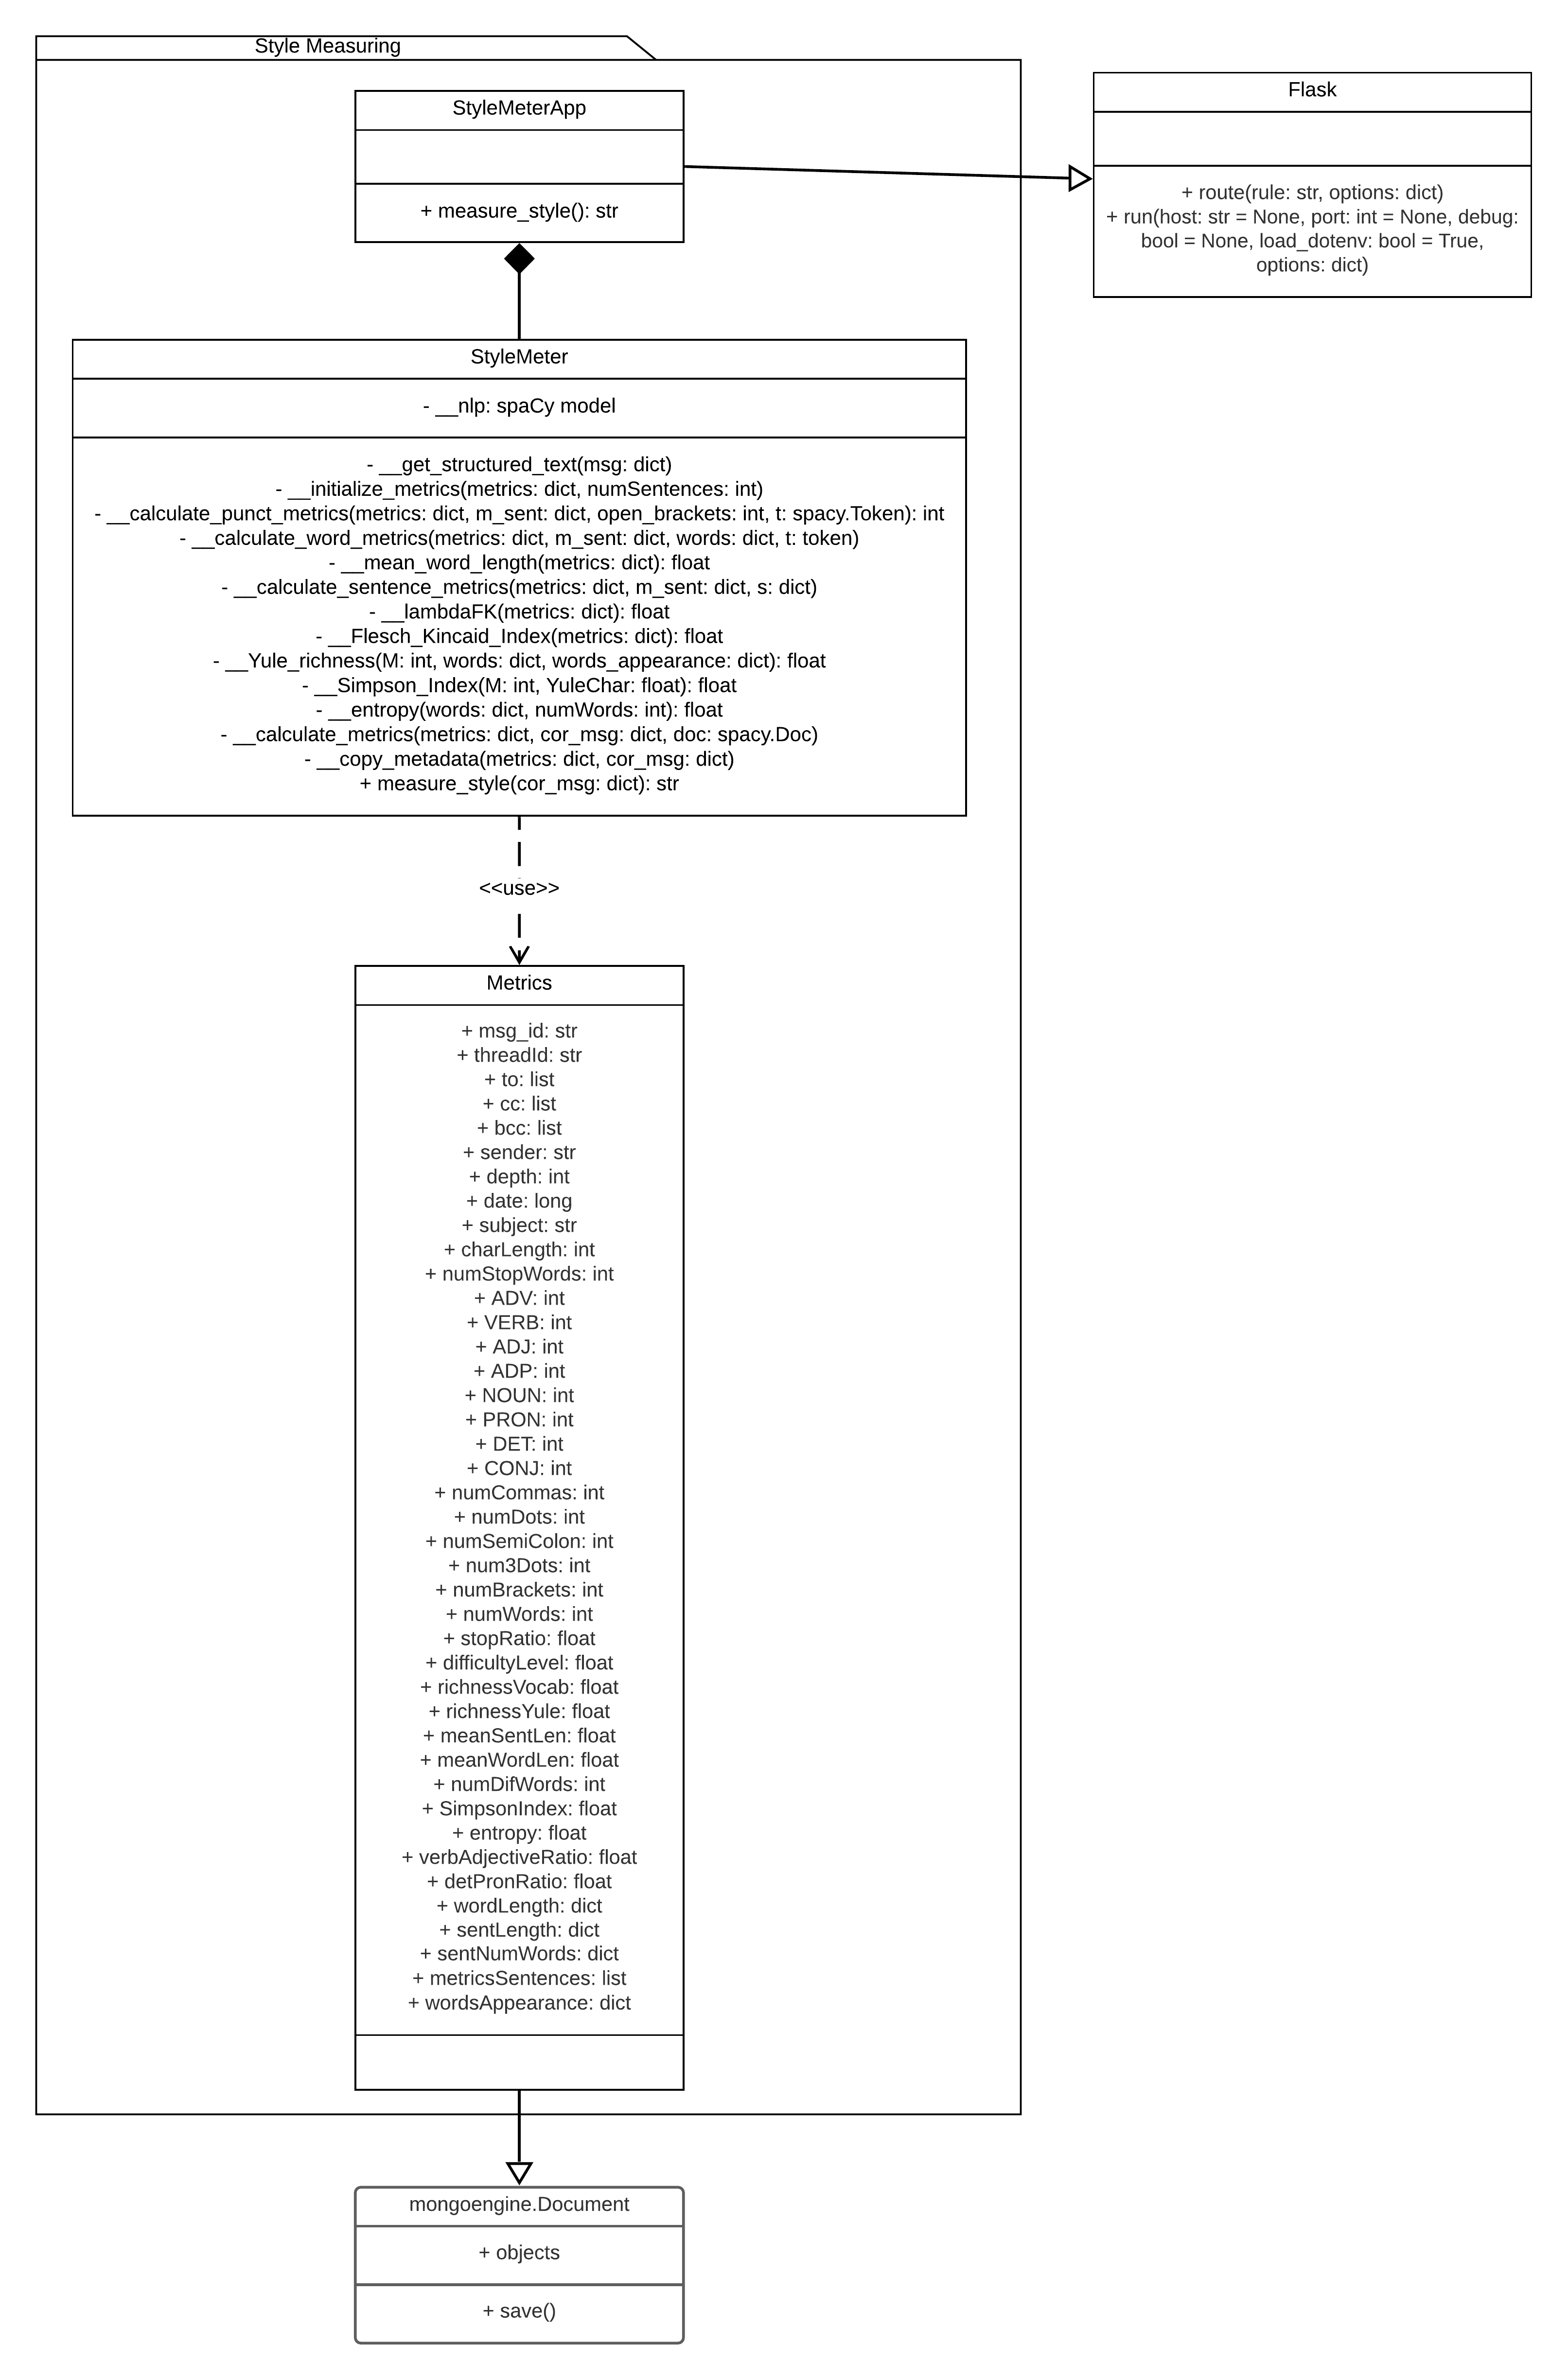
\includegraphics[height=0.85\paperheight]{Imagenes/Bitmap/Analyser/metUML.png}}%
	\caption{UML class diagram of the measuring module}%
	\label{fig:umlmet}
\end{figure}

As we can see in Figure \ref{fig:umlmet}, the style measuring package has three different classes with a class diagram similar to that of the preprocess package. These three classes are: \textit{StyleMeterApp}, \textit{StyleMeter} and \textit{Metrics}.

As with the two previous modules, this package implements a Flask web service which can be used through a POST HTTP request with the message as a \textit{json} in it. Having done so, the \textit{measure\_style} method of the \textit{StyleMeterApp} class will be invoked and send the given message structure to the \textit{StyleMeter} class by calling its only public method: \textit{measure\_style}.

The main class of this UML package is the \textit{StyleMeter} class. It is in charge of calculating the style features. For this reason, it has different methods which implement the distinct style markers that it has to evaluate.

As the reader is able to deduce after presenting the previous sections, the \textit{Metrics} class will store in the database the results of measuring each message. The \textit{StyleMeter} class will use it once it has calculated all the style characteristics.

We have used 31 lexical-syntactic features (due to previous studies, such as \cite{homem2011authorship}, yield encouraging results with lexical-syntactic features), following the classification of \cite{abbasi2008writeprints} (which categorised stylistic features as lexical, syntactic, structural, content-specific and idiosyncratic style markers), and we will now divide them into four categories in which we have grouped them according to their usefulness in terms of what type of conclusions we can infer from each of them. These categories are: part of speech features (see Section \ref{ssect:posf}), punctuation features (see Section \ref{ssect:punctf}), vocabulary features (see Section \ref{ssect:vocabf}) and structural features (see Section \ref{ssect:strucf}). We must not confuse this latter category (which belongs to the lexical features of the classification given in \cite{abbasi2008writeprints}) with the structural metrics explained in \cite{abbasi2008writeprints}. Some of the popular metrics which are not used in this work, belong to the structural, content-specific and idiosyncratic style markers of \cite{abbasi2008writeprints}, but there are others which belong to the same categories as the explained metrics (lexical and syntactic).

The choice of the metrics presented below, some essentially simple, has been directed by the objective of finding easily explainable characteristics that set the parameters of the style of writing according to the recipient of the e-mail, and then be able to use this study to develop, in future projects, systems of natural language generation of e-mails that take into account this factor. For this reason, some excessively complex metrics, although popular in stylometry, have been avoided and an attempt has been made to prioritize the explainability of the chosen features.

Finally, we are going to relate the explained style markers with their implementation (see Section \ref{ssect:relmet}) in the \textit{Metrics} class.

\subsection{Part of Speech features}\label{ssect:posf}

We will call our part of speech metrics as the syntactic features which have to do with the part of speech of each word of the e-mails. Following the suggestion of \cite{holmes1985analysis}, we count the number of nouns, verbs, adjectives, adverbs, pronouns, determinants, conjunctions and prepositions of each text. By calculating this, significant stylistic traits may be found, because as \cite{somers1966statistical} claims: ``A more cultivated intellectual habit of thinking can increase the number of substantives used, while a more dynamic empathy and attitude can be habitually expressed by means of an increased number of verbs. It is also possible to detect a number of idiosyncrasies in the use of prepositions, subordinations, conjunctions and articles''.

In addition to this metrics, we calculate the verb-adjective ratio and the determinant-pronouns ratio, extracted from \cite{antosch1969diagnosis} and \cite{brainerd1974weighting}, respectively.

\subsection{Punctuation features}\label{ssect:punctf}

In order to extract conclusions from this syntactic features, and following the example of \cite{calix2008stylometry}, we calculate the amount of commas, periods, semi-colons, ellipsis and pair of brackets. With these metrics we can reach conclusions such as the structural complexity of a message (since, for example, juxtaposition structures appear in the presence of some of these scores), the division into sentences of the message or the need for clarification of the text transmitted (for example, by analysing the amount of brackets).

\subsection{Vocabulary features}\label{ssect:vocabf}

In terms of the used vocabulary, we work with the ``bag of words'' metrics, in other words, we note how many times each different word is used in a message. Of course this is not the only metric that we can categorise as a vocabulary feature and from which we can extract conclusions about the vocabulary used. There are many others which try to set the parameters of, for instance, the difficult of the vocabulary or its richness. Furthermore, from the computing of the bag of words, we are able to easily obtain other style marker chosen which also belongs to this category of vocabulary features: the amount of different words in each text, proposed in \cite{ril2014determination} and in \cite{corney2001identifying}.

As for the difficulty level, it determines the level of education that someone needs to have if they are to understand the text. There are several indices available to calculate this level, such as the proposed in \cite{dale1948formula}, the Gunning Fog Index \citep{wiki:gunning} or the Flesch-Kincaid index \citep{dubay2004principles}, although the latter is the most commonly documented and cited. The expression which determines the Flesch-Kincaid index is the following:

$$
I_{FK} = 1.599\lambda-1.015\beta-31.517
$$

Where $\lambda$ is the mean of one-syllable words per 100 words, and $\beta$ is the mean sentence length measured by the number of words. However, as our spaCy's pretrained Spanish model (see Section \ref{sect:spacy}) is not able to divide words by syllables, we determine $\lambda$ as the mean of words with two or less characters per 100 words.

In respect of the richness of the vocabulary, we have chosen two different metrics. The first that we are going to explain is the one proposed by \cite{honore1979some}, which determines the richness of the vocabulary based on the total unrepeated words used in the text. The following formula defines it:

$$
R_H = \frac{100\log(M)}{M^2}
$$

Where $M$ is the number of different words in the text. However, as \cite{ril2014determination} claims, depending on the type of document being analysed, the calculation of $R_H$ has more or less validity (for instance, certain specialist articles, as their nature, requires constant repetition of words). As a consequence of this, another definition of richness of vocabulary is proposed by \cite{yule2014statistical}. This richness marker, that we are going to use as our second richness of vocabulary style marker, is called Yule's characteristic and defined with the following expression:

$$
K = \frac{10^4\left(\sum_{i = 1}^\infty i^2V_i-M\right)}{M^2}
$$

Where $M$ is the number of different words in the text and $V_i$ is the number of words that appear i times in the document.

From Yule's Characteristic we are able to calculate the Simpson's Index (denoted as $D$), defined in \cite{simpson1949measurement}. This famous metric is understood as the measurement of diversity based on the change that the two members of an arbitrary chosen pair of word tokens will belong to the same type. To calculate $D$ it is necessary to divide the total number of identical pairs in the sample by the number of all possible pairs, that is to say, what the following expression defines:

$$
D = \frac{\sum_{i = 1}^\infty i(i-1)V_i}{M(M-1)}
$$

Where we are maintaining the Yule's Characteristic notation. However, as we have transmitted in advance, it is possible to calculate the Simpson's Index if we know the value of Yule's Characteristic. This relationship is defined by the following expression (and we are going to use it in the implementation in order to speed the computing):

$$
10^{-4}K=D\left(1-\frac{1}{M}\right)
$$

Vocabulary distribution can also be measured by using a concept linguists have borrowed from thermodynamics and applied to communication theory: entropy (used in \cite{holmes1985analysis}). In literary text it is true that with an increase in internal structure, entropy decreases, and with an increase in disorder or randomness, the measure of entropy increases. The expression for the entropy of a system (vocabulary in this case) is:

$$
H = -\sum_{i=1}^{\infty} p_i\log(p_i)
$$

Where $p_i$ is the probability of appearance of the ith lemma (found by dividing the number of occurrences of that lemma by the total number of words in the text). Due to the value will change according to how much text is analysed, the formula may be refined in order that works of different length may be compared. In this way, as it is proposed in \cite{holmes1985analysis}, the following expression determines absolute diversity for any length text as 100, while absolute uniformity remains zero:

$$
H=-100\sum_{i = 1}^{\infty}p_i\frac{\log(p_i)}{\log(M)}
$$

In addition to the words distribution features (which are the bag of words and the amount of different words), the level of difficulty, the richness of vocabulary (which is measured by the formula proposed in \cite{honore1979some} and the Yule's Characteristic), the diversity (represented by the Simpson's Index) and the internal structure of the vocabulary (which is measured by the entropy), we have defined other four style markers which also allow us to extract conclusions about some feature of the vocabulary of the message. The first of these is the most popular and old style marker: the mean word length. Researchers as \cite{ril2014determination} claim that it is ``directly connected with the richness of the author's vocabulary and measures his or her ability to use complex words'', due to it is considered that complex words are formed by three or more syllables that do not represent proper nouns, prefixes, suffixes or compound words. Thus, \cite{ril2014determination} propose an expression similar to the following one in order to calculate it:

$$
L_W = \frac{\sum_{i=1}^{\infty}i*C_i}{N}\cdot 100
$$

Where $C_i$ is the number of words with $i$ characters and $N$ is the number of words used. This formula is analogous to the expression proposed by \cite{ril2014determination}, except that with the one that we have presented the punctuation marks are removed from the numerator.

The second of these writing style metrics is the measurement of words length frequency distribution, that is to say, how many words with one character appear in the document, with two characters and so on up to the length of the longest word. Despite of being strongly influenced by the language, it is used in researches as \cite{corney2001identifying} and \cite{kemp1976personal}, as it is claimed in \cite{allen1974methods}: ``Each writer, however, will have his own curve, so that although English (and German) texts in general peak at three letters, the writings of John Stuart Mill peak at two and those of Shakespeare peak at four''. Our interest will then focus on checking whether, in addition to depending on the author, this metric varies according to the recipient of the e-mail.

The rest of vocabulary features are related to the stop words present in the text. The simplest of those metrics is the style marker which consists of calculating the total number of stop words (denoted as $T_S$). On the other hand, as it is proposed in \cite{ril2014determination},  we will calculate the stop words ratio, which is defined with the following expression:

$$
S_W = \frac{T_S}{N}\cdot 100
$$

\subsection{Structural features}\label{ssect:strucf}

We will denote by structural features those characteristics that we obtain directly from the construction of the analysed text. Some of these metrics are as simple as the total number of characters in the body of the e-mail or the absolute number of words in the e-mail, both used in researches such as in \cite{corney2001identifying} and \cite{ril2014determination}.

Most of these features are sentence length dependent. Both \cite{tallentire1972appraisal} and \cite{kjetsaa1979and} agree that summary measures such as average sentence-lengths are of little use in stylometry studies but distributions of sentence-lengths can be useful, even on their own. Taking into account the above, we will find both the distribution of the length of the sentences (calculated in number of characters and number of words) and the average length of the sentences in a message found by the number of words, as it is proposed in \cite{corney2001identifying}. For the first one, we are going to store the number of sentence with length one, two, three and so on up to the length of the longest one, by measuring it  using both the number of characters and the number of words.

\subsection{Relationship between metrics and their implementation}\label{ssect:relmet}
Every explained style markers is stored as an attribute of the \textit{Metrics} class. The relationship between them and the presented style features and the categorisation of these metrics is exposed in Table \ref{tab:sty}.

\begin{table}[h]
	\begin{tabular}{|l|ll|}
		\hline
		\multicolumn{1}{|c|}{Feature Category} & \multicolumn{1}{l}{Field name} & \multicolumn{1}{l|}{Explanation}                    \\ \hline
		\multirow{10}{*}{Part of speech}       & ADV                            & Number of adverbs                                   \\ \cline{2-3} 
		& VERB                           & Number of verbs                                     \\ \cline{2-3} 
		& ADJ                            & Number of adjectives                                \\ \cline{2-3} 
		& ADP                            & Number of prepositions                              \\ \cline{2-3} 
		& NOUN                           & Number of nouns                                     \\ \cline{2-3} 
		& PRON                           & Number of pronous                                   \\ \cline{2-3} 
		& DET                            & Number of determinants                              \\ \cline{2-3} 
		& CONJ                           & Number of conjunctions                              \\ \cline{2-3} 
		& verbAdjectiveRatio             & Verb-adjective ratio                                \\ \cline{2-3} 
		& detPronRatio                   & Determinant-pronouns ratio                          \\ \hhline{|=|=|=|}
		\multirow{5}{*}{Punctuation}           & numCommas                      & Number of commas                                    \\ \cline{2-3} 
		& numDots                        & Number of periods                                   \\ \cline{2-3} 
		& numSemiColon                   & Number of semi-colons                               \\ \cline{2-3} 
		& num3Dots                       & Number of ellipsis                                  \\ \cline{2-3} 
		& numBrackets                    & Number of pair of brackets                          \\ \hhline{|=|=|=|}
		\multirow{11}{*}{Vocabulary}           & wordsAppearance                & Bag of words                                        \\ \cline{2-3} 
		& numDifWords                    & Number of different words                           \\ \cline{2-3} 
		& difficultyLevel                & Modified Flesch-Kincaid index ($I_{FK}$)                       \\ \cline{2-3} 
		& richnessVocab                  & \cite{honore1979some} vocabulary richness ($R_H$)                                     \\ \cline{2-3} 
		& richnessYule                   & Yule's characteristic ($K$)                               \\ \cline{2-3} 
		& SimpsonIndex                   & Simpson's index ($D$)                                     \\ \cline{2-3} 
		& entropy                        & Entropy ($H$)                                             \\ \cline{2-3} 
		& meanWordLen                    & Mean word length ($L_W$)                                    \\ \cline{2-3} 
		& wordLength                     & Word length distribution                            \\ \cline{2-3} 
		& numStopWords                   & Number of stop words                                \\ \cline{2-3} 
		& stopRatio                      & Percentage of stop words ($S_W$)                            \\ \hhline{|=|=|=|}
		\multirow{5}{*}{Structural}            & charLength                     & Number of characters                                \\ \cline{2-3} 
		& numWords                       & Number of words                                     \\ \cline{2-3} 
		& sentLength                     & Sentence length distribution (number of characters) \\ \cline{2-3} 
		& sentNumWords                   & Sentence length distribution (number of words)      \\ \cline{2-3} 
		& meanSentLen                    & Average word count per sentence                     \\ \hline
	\end{tabular}
\caption{Classification of the style markers}\label{tab:sty}
\end{table}

There is only one attribute that we have not mentioned and does not appear in Table \ref{tab:sty}: \textit{metricsSentences}. This attribute is a list of as many items as there are sentences in the document and each of them has the following dictionary structure:

\begin{python}
{
	'numStopWords': int,
	'ADV': int,
	'VERB': int,
	'ADJ': int,
	'ADP': int,
	'NOUN': int,
	'PRON': int,
	'DET': int,
	'CONJ': int,
	'numCommas': int,
	'numDots': int,
	'numSemiColon': int,
	'num3Dots': int,
	'numBrackets': int,
	'wordLength':
	{
		'1': int,
		'2': int,
		...
	}
	'charLength': int,
	'numWords': int,
	'stopRatio': float,
	'meanWordLen': float
}
\end{python}

With this dictionary, we calculate these metrics for each sentence, instead of evaluating them on the entire message.

\section{Analyser class}\label{sect:analyserclass}
The \textit{Analyser} class in charge of managing all phases in the pipeline, in other words, it sends to each module the required input in order to obtain its output. Besides, as it has been explained in Section \ref{section:typomod}, where the typographic correction module was presented, it asks the user the necessary information for the purpose of detecting and correcting, if it is required, the found typographic errors. In addition to it, as we can see in Figure \ref{fig:umlanalyser}, this class is able to store information in the database and extract it through the \textit{SessionTypoError} class.

\begin{figure}[h]
	\centering%
	\centerline{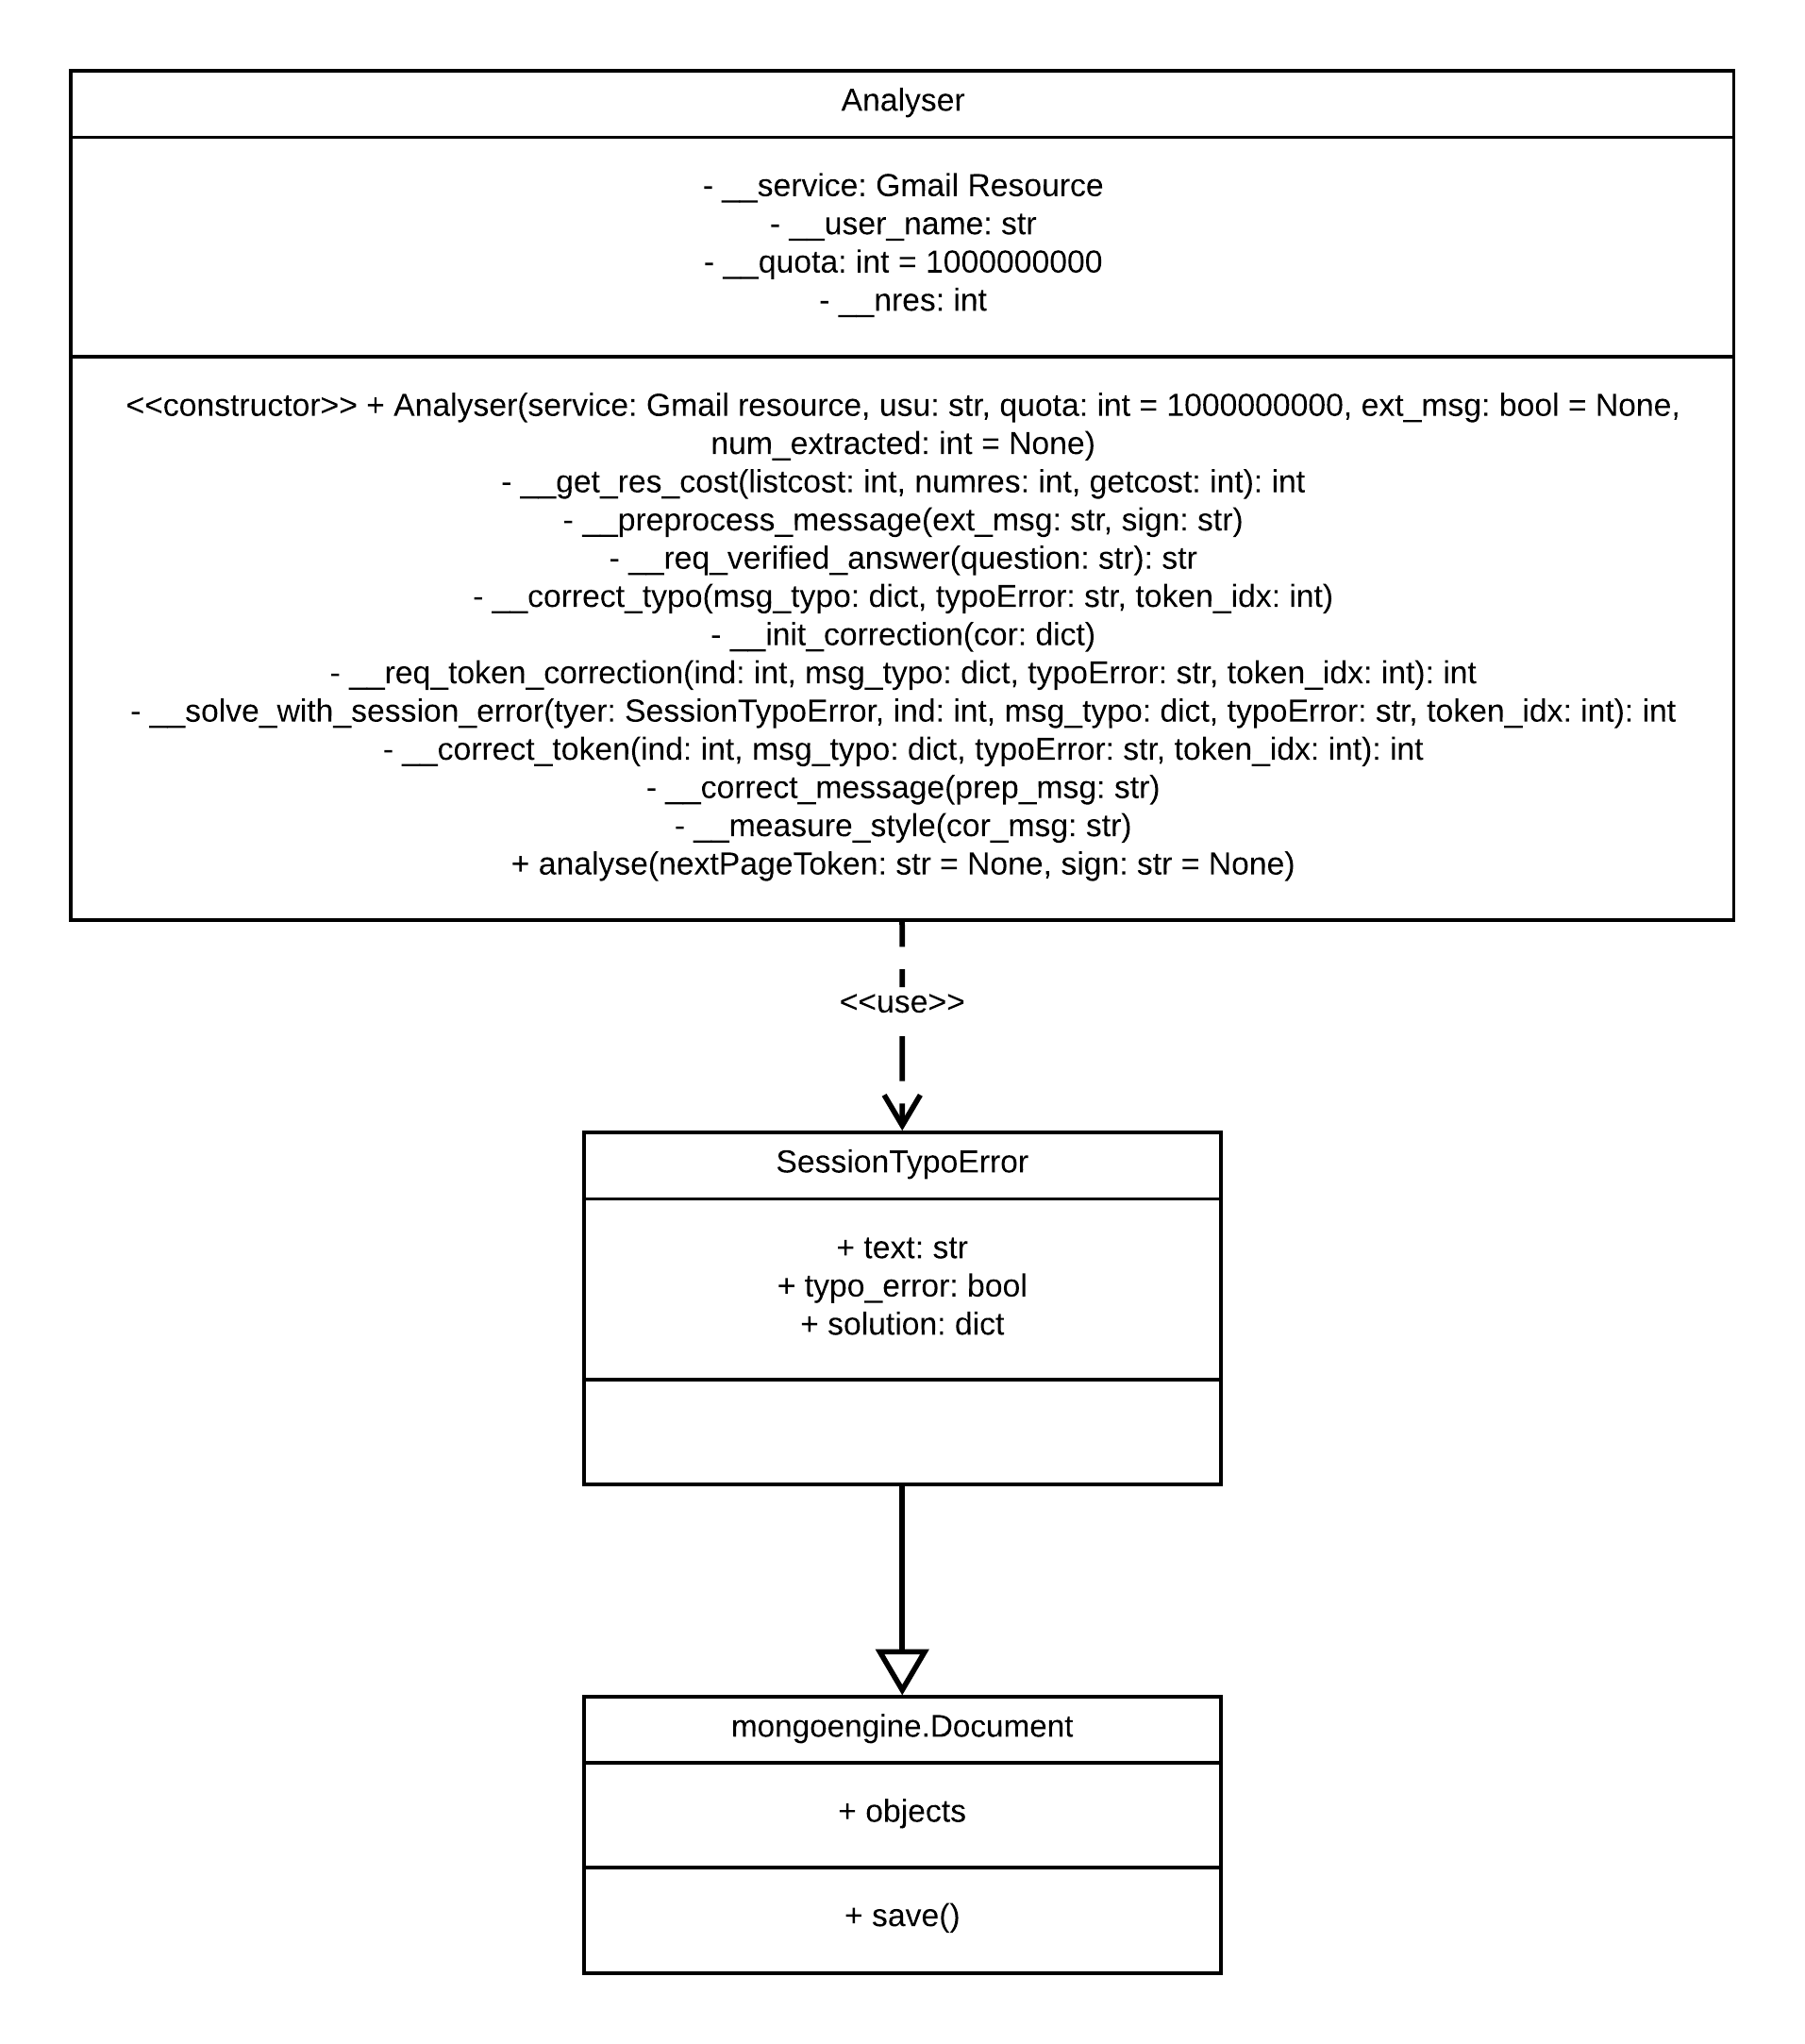
\includegraphics[width=0.6\paperwidth]{Imagenes/Bitmap/Analyser/analyserUML.png}}%
	\caption{UML class diagram of the Analyser}%
	\label{fig:umlanalyser}
\end{figure}

The \textit{Analyser}'s class constructor has an special interest in this system, due to it chooses the type of extraction that is going to be executed: a message extraction or a thread extraction. With the purpose of making this choice, the \textit{get} method of the labels resource is invoked in order to obtain the value of the fields \textit{messagesTotal} and \textit{threadsTotal} of the \textit{SENT} label structure (see Section \ref{sssect:labres}). With this values tha \textit{Analyser} is able to calculate the quota units cost (as we see in Section \ref{section:extmod}) of each type of extraction (this task is carried out by the \textit{\_\_get\_res\_cost} method) and choose the one which minimises it. After deciding it, it gives effect to the choice by creating the corresponding object with the type of extraction (\textit{MessageExtractor} or \textit{ThreadExtractor}).

Once an \textit{Analyser} object is created, the entire system can start its execution by calling the \textit{analyse} function (the web services of the modules which represent the last three phases in the pipeline have to be running). During the execution of this method, the only module that could require the attention of the \textit{Analyser} is the typographic correction module. The rest of the packages only need this class to provide the input messages and collect their output structures.

If the \textit{TypoCorrector} detects a typographic error, the first action that the \textit{Analyser} carries out is searching in the database if that word was previously found and corrected. For this purpose, the \textit{SessionTypoError} stores the common typographic errors that a user made (this collection is dropped at the beginning of each execution) and how to solve it (the \textit{solution} field has the same structure as the items of the list \textit{corrections} of the structure given by the \textit{TypoCorrector}). If it is a real typographic error, the \textit{typo\_error} field will take the value \textit{True} and in the \textit{solution} dictionary the text that should replace the word is stored. If it is not, the \textit{solution} dictionary will be appended to the \textit{corrections} list and the message will go on being corrected.

In the case that this typographic error is not stored, the \textit{Analyser} will ask the user whether the message has to be discarded (this option allows the user to remove from the pipeline, for instance, e-mail written in other languages). If it is discarded, the \textit{Analyser} sends then next message ready to be corrected to the typographic correction module. If it is not discarded, the \textit{\_\_req\_token\_correction} method is invoked. This function asks the user whether the word is a real typographic error. If it is, there are two solutions: to remove the token from the text or to rewrite it. Either way, at the end the user is going to answer the question: ``Do you want to save this information for this session?'' In this way the user will decide whether the solution is inserted in the collection managed by \textit{SessionTypoError} in case the same error is detected again.

If it is not a real typographic error, the user will answer some questions about the token: such as whether it is an url, an e-mail, a punctuation mark, a stop word, what its part of speech is and what its lemma is. Then, this information is appended to the \textit{corrections} list and ask the user whether this information is stored in \textit{Correction} collection for the future or in \textit{SessionTypeError} collection for this session.

Once the detected word is managed, the \textit{Analyser} resends the message to the typographic correction module in order to go on correcting it.



\section{Execution behaviour} \label{section:exebehav}
After executing it with the Gmail account that is analysed (the author's Gmail account), of the 1084 e-mails extracted, 921 were measured, which represents approximately the $84.96$\% of the total. In this execution, all the 1084 messages were correctly preprocessed, but 163 were discarded in the typographic correction phase. Some of them were discarded because, after the preprocessing, they were missing text, whereas the rest of them did not pass this phase due to its language (there were e-mails written in English) or, a minority because they had a not interested message body for the analysis of the writing style (for example we found some e-mails whose only text was an url).

\section{Conclusions}
In order to measure all the e-mails of a user, we develop a style analyser which has four different phases: extraction (which makes use of Gmail API with the purpose of extracting all the sent messages), preprocessing (which is in charge of transforming the body of the e-mail so the spaCy model can analyse it, for instance by removing the signature or soft break lines introduced due to the message encoding), typographic correction (which detects and corrects the typographic mistakes) and style measuring (which calculates the value of different metrics of each e-mail). The modules which correspond to the last three phases are implemented as web services so they are easily reusable in other projects. Besides, each module is independent to the rest of them. For this reason, it is necessary an \textit{Analyser} class in charge of assembling all these different packages.

After executing the style analyser with a Gmail account, we obtain the metrics of 921 messages. With these results, we can study the effectiveness of each metric to distinguish the different recipients of the messages. In the next chapter, we try to draw conclusions about the obtained metrics.